\documentclass[oneside,a4paper,11pt]{book}
\usepackage[utf8]{inputenc}
\usepackage{svg}
\usepackage[italian]{babel}
\usepackage{float}
\usepackage{fancyvrb}
\usepackage{titling}
\usepackage[margin=1in,footskip=0.25in]{geometry}
\usepackage{listings}
\usepackage[DIV=12,BCOR=2mm,headinclude=true,footinclude=false]{typearea}
\usepackage{color, colortbl,xcolor}
\usepackage[hidelinks]{hyperref}
\usepackage{tcolorbox}
\usepackage{chngcntr}
\usepackage{diagbox}
\usepackage{calc}
\usepackage{amssymb}
\usepackage{subcaption}
\usepackage{amsthm}
\usepackage{amsfonts}
\usepackage{mathtools}
\usepackage{parskip}
\usepackage{cancel}
\usepackage{forest}
\usepackage{listings}
\usepackage{mathrsfs}
\usepackage{enumitem}
\usepackage{makecell}
%TIKZ environment
\usepackage{tikz}
\usepackage{pgfplots}
\pgfplotsset{compat=1.18}
\usepackage{fancyhdr}
\fancypagestyle{plain}{\fancyhf{}\renewcommand{\headrulewidth}{0pt}} % To clear page numbers from footer, and header line at the start of every chapter

\pagestyle{fancy}
\fancyhf{}% Clear header/footer
\fancyhead[L]{\nouppercase\leftmark}
\fancyhead[R]{\thepage}


\usetikzlibrary{positioning,shapes.geometric,arrows.meta,matrix,automata,decorations.pathmorphing,patterns,decorations.pathreplacing,shapes.multipart,calc,snakes}
\usetikzlibrary{arrows.meta,
                backgrounds,
                chains,
                positioning,
                shapes.geometric, shapes.multipart
                }
\tcbuselibrary{skins}
\counterwithin{figure}{section}
%Nuovi comandi
\newcommand\myeq{\stackrel{\mathclap{\normalfont\mbox{def}}}{=}}
\newcommand\prodG{\stackrel{\mathclap{\normalfont\mbox{\tiny{G}}}}{\Longrightarrow}}
%asmthm
\newlength{\marginlabelsep}\setlength{\marginlabelsep}{0.5em}
\newtheoremstyle{italicstyle} %% Name
  {} %% <- Space above (empty = default = \topsep = 8.0pt plus 2.0pt minus 4.0pt)
  {} %% <- Space below (empty = default = \topsep = 8.0pt plus 2.0pt minus 4.0pt)
  {\itshape} %% <- Body font
  {} %% <- Indent amount (empty = no indent, \parindent = just that)
  {\bfseries} %% <- Thm head font
  {} %% <- Punctuation after thm head
  {1pt} %% <- Space after thm head (or " " or \newline) (default: 5pt plus 1pt minus 1pt)
  {\vtop to 0pt{\llap{\thmname{#1}\hskip\marginlabelsep}
                \llap{\thmnumber{#2}\hskip\marginlabelsep}}\thmnote{#3\\}%
  }
\newtheoremstyle{normStyle} %% Name
  {} %% <- Space above (empty = default = \topsep = 8.0pt plus 2.0pt minus 4.0pt)
  {} %% <- Space below (empty = default = \topsep = 8.0pt plus 2.0pt minus 4.0pt)
  {\normalfont} %% <- Body font
  {} %% <- Indent amount (empty = no indent, \parindent = just that)
  {\bfseries} %% <- Thm head font
  {} %% <- Punctuation after thm head
  {1pt} %% <- Space after thm head (or " " or \newline) (default: 5pt plus 1pt minus 1pt)
  {\vtop to 0pt{\llap{\thmname{#1}\hskip\marginlabelsep}
                \llap{\thmnumber{#2}\hskip\marginlabelsep}}\thmnote{#3\\}%
  }
\theoremstyle{italicstyle}
\newtheorem{corollary}{Corollario}[section]
\newtheorem{notazione}{Notazione}[section]
\newtheorem{lemma}{Lemma}[section]
\newtheorem{definizione}{Definizione}[section]
\newtheorem{nota}{Nota}[section]
\newtheorem{exercise}{Esercizio}[section]

\theoremstyle{normStyle}
\newtheorem{exmp}{Esempio}[section]
\newtheorem{theorem}{Teorema}[section]
\newtheorem{proposizione}{Proposizione}[section]

\tcbuselibrary{listings,skins}
\newtcblisting{mylisting}[2][]{
        arc=0pt, outer arc=0pt,
    listing only, 
    title=#2,
    #1,
    listing options= {escapechar=|}
}
%% global declaration
\RequirePackage{tikz}
\RequirePackage{ifthen}

% use libraries
\usetikzlibrary{arrows,shapes,snakes,matrix}


%% global declaration
\tikzstyle{btreeptr} = [draw, semithick, minimum height=2em]
\tikzstyle{btreeval} = [draw, semithick, minimum size=2em]
\tikzstyle{btreevale} = [draw,semithick, minimum size=2em]
\tikzstyle{btlink} = [draw, semithick, ->, >=triangle 45]
%% macro
%% helper macros
\newcommand{\suppressemptystr}[1]{% leave blank for entries in leaf nodes
  \ifthenelse{\equal{#1}{}}%
  {%
    \relax%
  }%
  % Else
  {%
    #1\textsuperscript{*}%
  }%
}%

\newcommand{\xyshift}[3]{% help to place the nodes
  \begin{scope}[xshift=#1, yshift=#2]
    #3
  \end{scope}%
}

%% Common btree macros
\newcommand{\btreelink}[2]{% #1: src node; #2: dest node; 
  \draw[btlink] ([yshift=3pt] #1.south) -- (#2-b.north);
}

\newcommand{\btreelinknorth}[2]{% #1: src node; #2: dest node; 
  \draw[btlink] ([yshift=3pt] #1.south) -- (#2.north);
}

\newcommand{\btreetriangle}[2]{% #1: node name; #2 text inside
  \node[anchor=north, regular polygon, regular polygon sides=3, draw] (#1) {#2};
}
%%======================================================================
%% btree with capacity = 1
\newcommand{\btreeinodeone}[2]{%
  \matrix [ampersand replacement=\&] (#1)
  {
    \node[btreeptr] (#1-1) {\vphantom{1}}; \& \node[btreeval] (#1-a) {#2}; \&
    \node[btreeptr] (#1-2) {\vphantom{1}}; \\
  };
}
\newcommand{\btreelnodeone}[2]{%
  \matrix [ampersand replacement=\&, outer sep=0pt, matrix anchor=north] (#1)
  {
    \node[btreevale] (#1-a) {\suppressemptystr{#2}}; \\
  };
}
%%=======================================================================
\newcommand{\btreeinodefour}[5]{%
  \matrix [ampersand replacement=\&] (#1)
  {
    \node[btreeptr] (#1-1) {\vphantom{1}}; \& \node[btreeval] (#1-a) {#2}; \&
    \node[btreeptr] (#1-2) {\vphantom{1}}; \& \node[btreeval] (#1-b) {#3}; \&
    \node[btreeptr] (#1-3) {\vphantom{1}}; \& \node[btreeval] (#1-c) {#4}; \&
    \node[btreeptr] (#1-4) {\vphantom{1}}; \& \node[btreeval] (#1-d) {#5}; \&
    \node[btreeptr] (#1-5) {\vphantom{1}}; \\
  };
}
\newcommand{\btreelnodefour}[5]{%
  \matrix [ampersand replacement=\&, outer sep=0pt, matrix anchor=north] (#1)
  {
    \node[btreevale] (#1-a) {\suppressemptystr{#2}}; \&
    \node[btreevale] (#1-b) {\suppressemptystr{#3}}; \&
    \node[btreevale] (#1-c) {\suppressemptystr{#4}}; \&
    \node[btreevale] (#1-d) {\suppressemptystr{#5}}; \\
  };
}
%%======================================================================
%% btree with capacity = 2
\newcommand{\btreeinodetwo}[3]{%
  \matrix [ampersand replacement=\&] (#1)
  {
    \node[btreeptr] (#1-1) {\vphantom{1}}; \& \node[btreeval] (#1-a) {#2}; \&
    \node[btreeptr] (#1-2) {\vphantom{1}}; \& \node[btreeval] (#1-b) {#3}; \&
    \node[btreeptr] (#1-3) {\vphantom{1}}; \\
  };
}
\newcommand{\btreelnodetwo}[3]{%
  \matrix [ampersand replacement=\&, outer sep=0pt, matrix anchor=north] (#1)
  {
    \node[btreevale] (#1-a) {\suppressemptystr{#2}}; \&
    \node[btreevale] (#1-b) {\suppressemptystr{#3}}; \\
  };
}

%%======================================================================
%% btree with capacity = 3
\newcommand{\btreeinodethree}[4]{%
  \matrix [ampersand replacement=\&] (#1)
  {
    \node[btreeptr] (#1-1) {\vphantom{1}}; \& \node[btreeval] (#1-a) {#2}; \&
    \node[btreeptr] (#1-2) {\vphantom{1}}; \& \node[btreeval] (#1-b) {#3}; \&
    \node[btreeptr] (#1-3) {\vphantom{1}}; \& \node[btreeval] (#1-c) {#4}; \&
    \node[btreeptr] (#1-4) {\vphantom{1}}; \\
  };
}
\newcommand{\btreelnodethree}[4]{%
  \matrix [ampersand replacement=\&, outer sep=0pt, matrix anchor=north] (#1)
  {
    \node[btreevale] (#1-a) {\suppressemptystr{#2}}; \&
    \node[btreevale] (#1-b) {\suppressemptystr{#3}}; \&
    \node[btreevale] (#1-c) {\suppressemptystr{#4}}; \\
  };
}
%%======================================================================

\definecolor{xmlstring}{RGB}{42,0.0,255}
\definecolor{xmlcomment}{RGB}{50,128,50}

\lstdefinelanguage{XML}{
  %basicstyle=\ttfamily\small,
  basicstyle=\fontsize{9}{10}\selectfont\ttfamily,
  morestring=[b]",
  moredelim=[s][\bfseries\color{black}]{<}{\ },
  moredelim=[s][\bfseries\color{black}]{</}{>},
  moredelim=[l][\bfseries\color{black}]{/>},
  moredelim=[l][\bfseries\color{black}]{>},
  morecomment=[s]{<?}{?>},
  morecomment=[s]{<!--}{-->},
  stringstyle=\color{xmlstring},
  commentstyle=\color{xmlcomment},
  showstringspaces=false,
  breaklines=true
}

\lstset{
  language=XML,
  extendedchars=true,
  breaklines=true,
  breakatwhitespace=true,
  emph={},
  emphstyle=\color{red},
  basicstyle=\ttfamily,
  showstringspaces=false,
  commentstyle=\color{blue}\upshape,
  keywordstyle=\color{black},
  stringstyle=\color{xmlstring},
  captionpos=b
}

\newcommand{\myboxedtext}[2][rectangle,draw]{%
        \tikz[baseline=-0.6ex] \node [#1]{#2};}%
\title{Basi di Dati \\ \large{modulo Tecnologie}}
\author{Alessio Gjergji}
\date{Anno accademico 2022 - 2023}

\begin{document}
\hypersetup{ %set true if you want colored links
    linktoc=all,     %set to all if you want both sections and subsections linked
    linkcolor=black,  %choose some color if you want links to stand out
}
\maketitle
\tableofcontents
\chapter{Transazioni}
\section{Tecnologie per le basi di dati}
Un DBMS (\textit{Database Management System}) o sistema di gestione dei basi 
di dati, è un sistema software in grado di gestire collezioni di dati che 
siano, grandi, condivise e persistenti, assicurando la loro affidabilità 
e privatezza.

Un DBMS in quanto sistema software deve essere \textbf{efficiente} ed \textbf{efficace}, 
caratteristiche dipendenti dalla bontà di progettazione della base 
di dati. Deve inoltre estendere la funzionalità del file system, garantendo la 
gestione di collezioni di dati presenti in memoria secondaria.
Una base di dati è quindi di una collezione di dati gestita da un DBMS.
\begin{figure}[H]
    \centering
    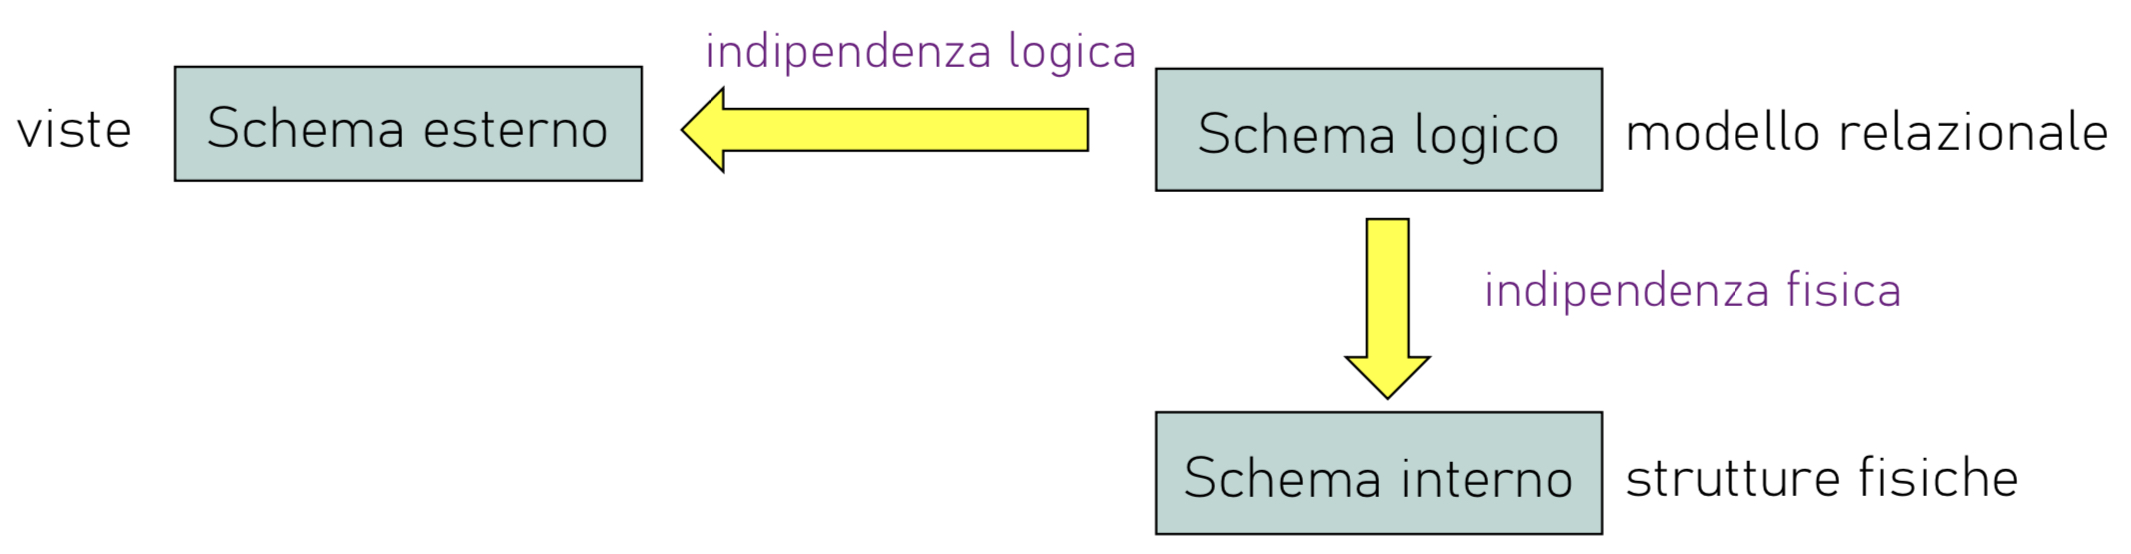
\includegraphics[width=15cm]{img/architetturaDBMS.jpeg}
    \caption{Tecnologia dei DBMS}
    \label{fig:tec_DBMS}
  \end{figure}
Un DBMS basato sul modello relazionale è nella maggior parte dei casi 
anche un \textbf{sistema transazionale}: fornisce quindi un meccanismo 
per la definizione ed esecuzione delle transazioni.
\subsection{Transazione}
\begin{tcolorbox}
La \textbf{transazione} è un'unità di lavoro svolta da un programma applicativo per 
la quale si vogliono garantire proprietà di correttezza, robustezza e isolamento.
\end{tcolorbox}
La principale caratteristica di una transazione è che solamente se va a buon fine 
ha effetto sulla base di dati, se non va a buon fine le operazioni vengono 
abortite, non sono quindi ammesse esecuzioni parziali.

La transazione va a buon fine all'esecuzione di un \verb|commit work|. Se 
Non ha alcun effetto sulla base di dati viene eseguito un \verb|rollback work|.

La transazione è ben formata se:
\begin{itemize}
    \item inizia con un \verb|begin transaction|;
    \item termina con un \verb|end transaction|;
    \item a sua esecuzione comporta il raggiungimento 
di un \verb|commit| o di un \verb|rollback work| senza che vengano eseguiti 
altri accessi alla base di dati successivamente. 
\end{itemize}
\subsubsection{Esempio}
\begin{lstlisting}
begin transaction;
    update CONTO set saldo = saldo - 1200
        where filiale = '005' and numero = 15;
    update CONTO set saldo = saldo + 1200
        where filiale = '005' and numero = 205;
    commit work;
end transaction;
\end{lstlisting}
\subsubsection{Proprietà delle transazioni}
Una transazione ha quattro proprietà:
\begin{itemize}
    \item Atomicità (\textit{Atomicity}): una transazione è una esecuzione 
    \textbf{indivisibile}. O viene eseguita completamente o non viene eseguita affatto.
    Se una transazione viene interrotta prima del commit, il lavoro fin qui 
    eseguito dalla transazione deve essere disfatto ripristinando la situazione in 
    cui si trovata la base di dati prima dell'inizio della transazione. Se 
    viene interrotta dopo l'esecuzione del commit, il sistema deve assicurare che 
    la transazione abbia effetto sulla base di dati.
    \item Consistenza (\textit{Consistency}): l'esecuzione di una transazione non deve 
    violare i \textbf{vincoli d'integrità}:
    \begin{itemize}
        \item Verifica immediata: fatta durante il la transazione, viene abortita solo 
        l'ultima operazione e il sistema restituisce all'applicazione una segnalazione 
        d'errore, l'applicazione può quindi reagire alla violazione.
        \item Verifica differita: al commit se un vincolo di integrità viene 
        violato, la transazione viene abortita senza possibilità da parte 
        dell'applicazione di reagire alla violazione.
    \end{itemize}
    \item Isolamento (\textit{Isolation}): l'esecuzione di una transazione deve essere 
    \textbf{indipendente} dalla contemporanea esecuzione di altre transazioni. Il rollback 
    di una transazione non deve creare rollback a catena di altre transazioni che 
    si trovano in esecuzione contemporaneamente. Il sistema, inoltre, deve
    regolare l'esecuzione concorrente con meccanismi di controllo dell'accesso 
    alle risorse.
    \item Persistenza (\textit{Durability}): l'effetto di una transazione che ha eseguito il commit
    non deve andar perso. Il sistema deve essere in grado, in caso di guasto, di garantire 
    gli effetti delle transazioni che al momento del guasto avevano già 
    eseguito un commit.
\end{itemize}
Un DBMS che gestisce transazioni dovrebbe garantire per ogni transazione 
che esegue tutte queste proprietà.
\subsection{Architettura di un DBMS}
L'architettura mostra i \textbf{moduli principali} che possiamo individuare nei DBMS attuali,
considerando le diverse funzionalità che il DBMS svolge durante l'esecuzione dell 
transazione.

Per ogni modulo dell'architettura presentiamo le \textbf{funzionalità} 
che esso svolge e alcune tecniche che applica.
\begin{figure}[H]
    \centering
    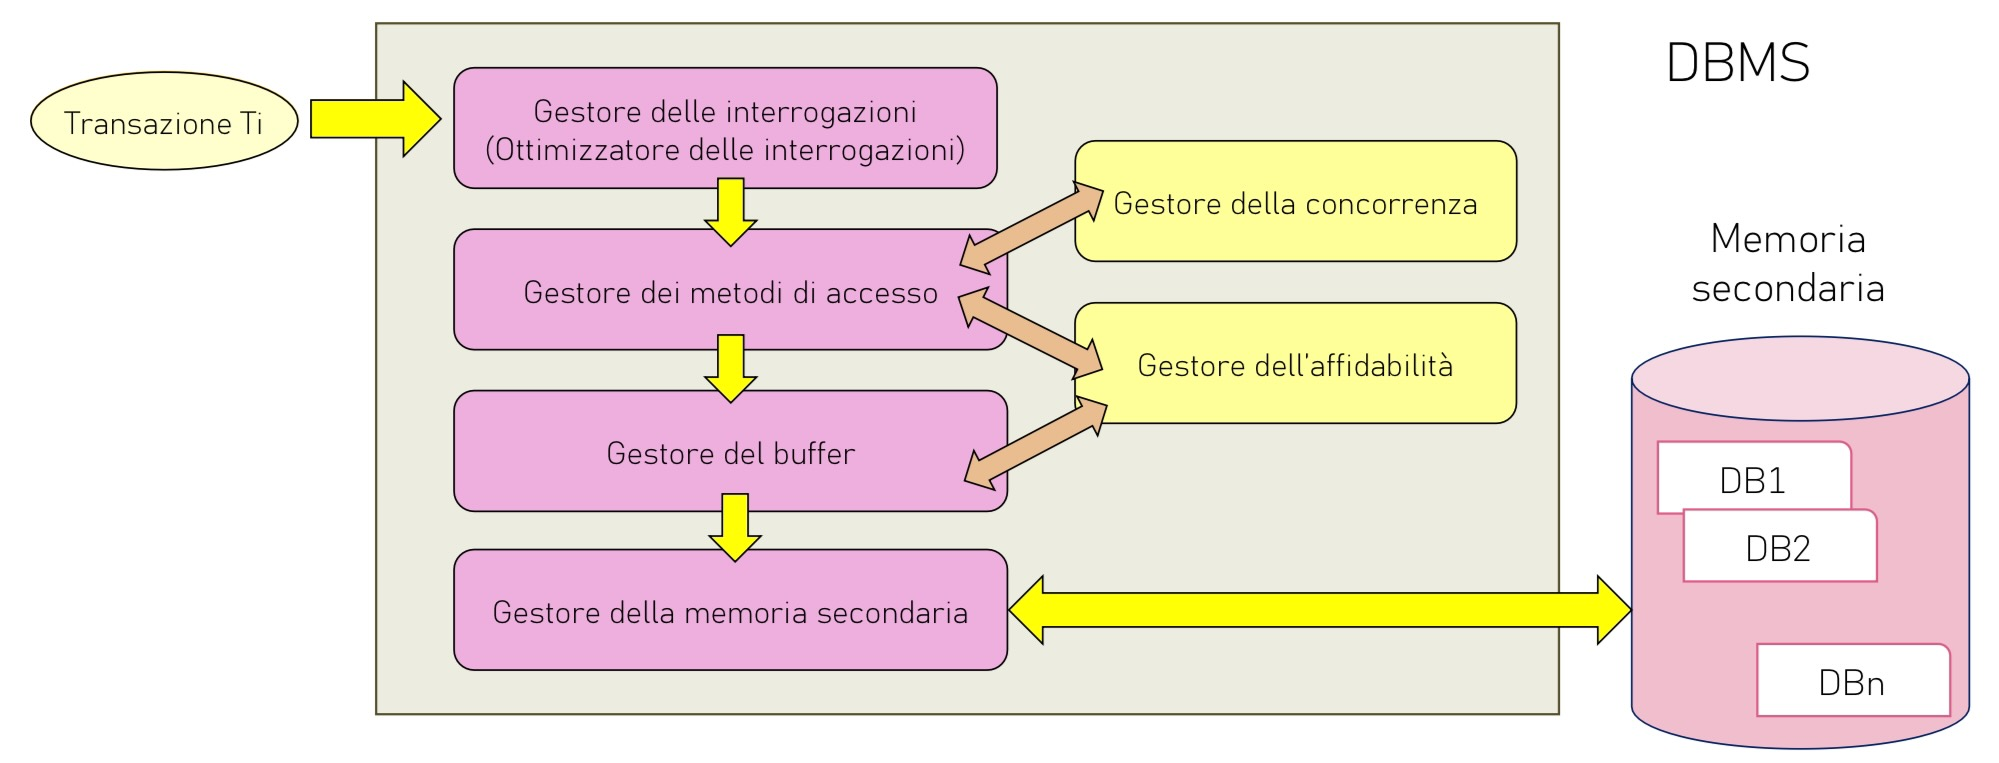
\includegraphics[width=15cm]{img/gestoriDBMS.jpeg}
    \caption{Architettura di riferimento di un DBMS}
    \label{fig:arhc_DBMS}
  \end{figure}
\subsubsection{Sequenza}
\begin{itemize}
    \item Il gestore delle interrogazioni prende in input una transazione, quindi 
    l'espressione DML e calcolerà un piano di esecuzione.
    \item Il piano di esecuzione sarà l'input per il gestore dei metodi 
    d'accesso, che eseguirà operazioni di:
    \begin{itemize}
        \item Richieste d'accesso verso il 
        gestore dell'esecuzione corrente.
        \item Riceverà permessi di accesso dal gestore dell'esecuzione 
        corrente
    \end{itemize}
    In output fornirà richieste di pagine (\textit{o blocchi della memoria 
    secondaria}) contenente dati e/o indici.
    \item  Le richieste di blocchi contenenti dati/indici sarà 
    l'input per il gestore dell'affidabilità (\textit{o dei guasti}) che manderà
    in output richieste di blocchi contenenti dati/indici o blocchi del \verb|LOG|.
    \item Le richieste di blocchi contenenti dati/indici o log andranno in 
    input al gestore del buffer, in comunicazione con la memoria secondaria.
\end{itemize}
I moduli che garantiscono le proprietà delle transazioni sono:
\begin{itemize}
    \item Gestore dei metodi d'accesso: consistenza.
    \item Gestore dell'esecuzione concorrente: atomicità e isolamento.
    \item Gestore dell'affidabilità: atomicità e persistenza. 
\end{itemize}
\section{Architettura di un DBMS}
Le basi di dati gestite da un DBMS risiedono in memoria secondaria, in 
quanto sono:
\begin{itemize}
    \item Grandi: non possono essere contenute in memoria centrale
    \item Persistenti: hanno un tempo di vita che non è limitato all'esecuzione 
    dei programmi che le utilizzano.
\end{itemize}
La memoria secondaria non è direttamente utilizzabile dai programmi, 
l'organizzazione dei dati è strutturata in pagine, le uniche operazioni 
possibili sono la lettura e la scrittura di un intera pagina e il costo 
di tali operazioni è in ordini di grandezza maggiore per accedere ai 
dati in memoria centrale.
\subsection{Gestore del Buffer}
L'interazione tra memoria secondaria e memoria centrale avviene attraverso 
il trasferimento di pagine della memoria secondaria in una zona appositamente 
dedicata della memoria centrale detta \textbf{buffer}. Tale zona è 
condivisa dalle applicazioni e quando uno stesso dato viene utilizzato 
più volte in tempi ravvicinati il buffer evita l'accesso alla memoria secondaria,
poiché dispendiosa. La gestione ottimale del buffer è strategica per ottenere 
buone prestazioni nell'accesso ai dati.
\begin{figure}[H]
    \centering
    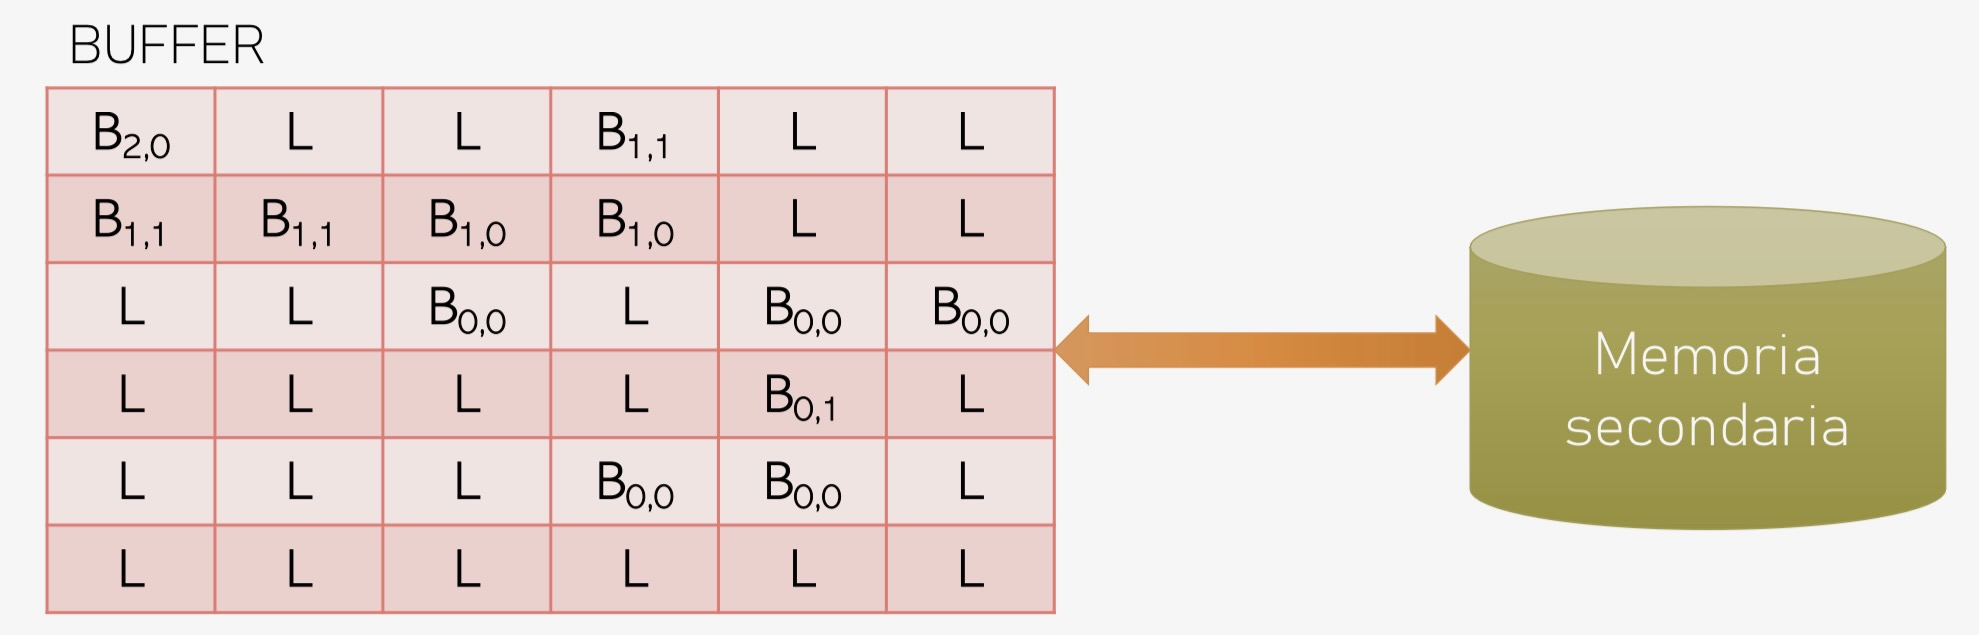
\includegraphics[width=15cm]{img/buffer.jpeg}
    \caption{$\texttt{B}_{i,j}$ indica che nella pagina del buffer è caricato 
    il blocco $\texttt{B}$, inoltre $\texttt{i}$ indica che il blocco è attualmente 
    utilizzato da $\texttt{i}$ transazioni, mentre $\texttt{j}$ è $1$ se il blocco è stato modificato,
    $0$ altrimenti. $\texttt{L}$ indica pagina libera.}
    \label{fig:buffer}
  \end{figure}
Il buffer è organizzato in pagine e una pagina ha le dimensioni di un blocco della memoria
secondaria. Il gestore del buffer si occupa del caricamento/salvataggio delle pagine in 
memoria secondaria a fronte di richieste di lettura/scrittura.
\subsubsection{Politica del gestore dei buffer}
\begin{itemize}
    \item Lettura di un blocco: se il blocco è presente in una pagina del buffer 
    allora non si esegue una lettura su memoria secondaria e si restituisce un puntatore 
    alla pagina del buffer. Altrimenti si cerca una pagina libera e si carica il blocco nella 
    pagina, restituendo il puntatore alla pagina stessa.
    \item Scrittura di un blocco: in caso di richiesta di scrittura 
    di un blocco precedentemente caricato in una pagina del buffer, il gestore del buffer può 
    decidere di differire la scrittura su memoria secondaria in un secondo momento.
\end{itemize}
In entrambi i casi l'obiettivo è quello di aumentare la velocità di 
accesso ai dati.

Tale comportamento del gestore dei buffer si basa sul \textbf{principio di località},
i dati referenziati di recente hanno maggiore probabilità di essere referenziati 
nuovamente in futuro.
Inoltre, una nota \textbf{legge empirica} dice che il $20\%$ dei dati e acceduto 
dall'$80\%$ delle applicazioni. 

Tutto ciò rende conveniente dilazionare la scrittura su memoria secondaria 
delle pagine del buffer.
\subsubsection{Gestione delle pagine}
Per ogni pagina del buffer si memorizza il \textbf{blocco B} contenuto 
indicando il file e l'offset del blocco. Per ogni pagina del buffer si memorizza un insieme di 
\textbf{variabili di stato} tra cui si trovano sicuramente:
\begin{itemize}
    \item Un contatore $\verb|i|$ per indicare il numero di transazioni che utilizzano 
    le pagine.
    \item Un bit di stato $\verb|j|$ per indicare se la pagina è stata modificata o meno.
\end{itemize}
\subsection{Primitive per la gestione del buffer}

La primitiva \verb|fix| viene usata dalle transazioni per richiedere l'accesso 
ad un blocco richiesto.

Passi della primitiva:
\begin{itemize}
    \item Il blocco richiesto viene cercato nelle pagine del buffer, in caso sia presente, si restituisce 
    un puntatore alla pagina contenente il blocco
    \item Altrimenti, viene scelta una pagina libera (\textit{in base a diversi criteri}) 
    e si carica il blocco aggiornando 
    file e numero di blocco corrispondenti.
    \item Se non esistono pagine libere, il gestore del buffer può adottare due politiche:
    \begin{itemize}
        \item Steal: ruba una pagina ad un'altra transazione (\textit{primitiva $\texttt{flush}$}).
        \item No Steal: sospende la transazione inserendola in una cosa d'attesa.
    \end{itemize}
\end{itemize}
Quando una transazione accede ad una pagina per la prima volta il contatore 
si incrementa.

La primitiva \verb|setDirty| viene usata dalle transazioni per 
indicare al gestore del buffer che il blocco della pagina è stato 
modificato. L'effetto è la modifica del bir di stato $\verb|J|$ a $1$.

La primitiva \verb|unfix| viene usata dalle transazioni per indicare che 
la transazione ha terminato di usare il blocco. L'effetto è il decremento 
del contatore $I$ che indica l'uso della pagina.

La primitiva \verb|force| viene usata per salvare in memoria secondaria 
in modo sincrono il blocco contenuto nella pagina. L'effetto è il 
salvataggio in memoria secondaria del blocco e il bit di stato $J$ posto a zero.

La primitiva \verb|flush| viene usata dal gestore del buffer per 
salvare blocchi sulla memoria secondaria in modo asincrono. Tale 
operazione libera \textit{dirty} (\textit{il bit di stato 
viene posto a zero}).
\subsection{Gestore dell'affidabilità}
\begin{figure}[H]
    \centering
    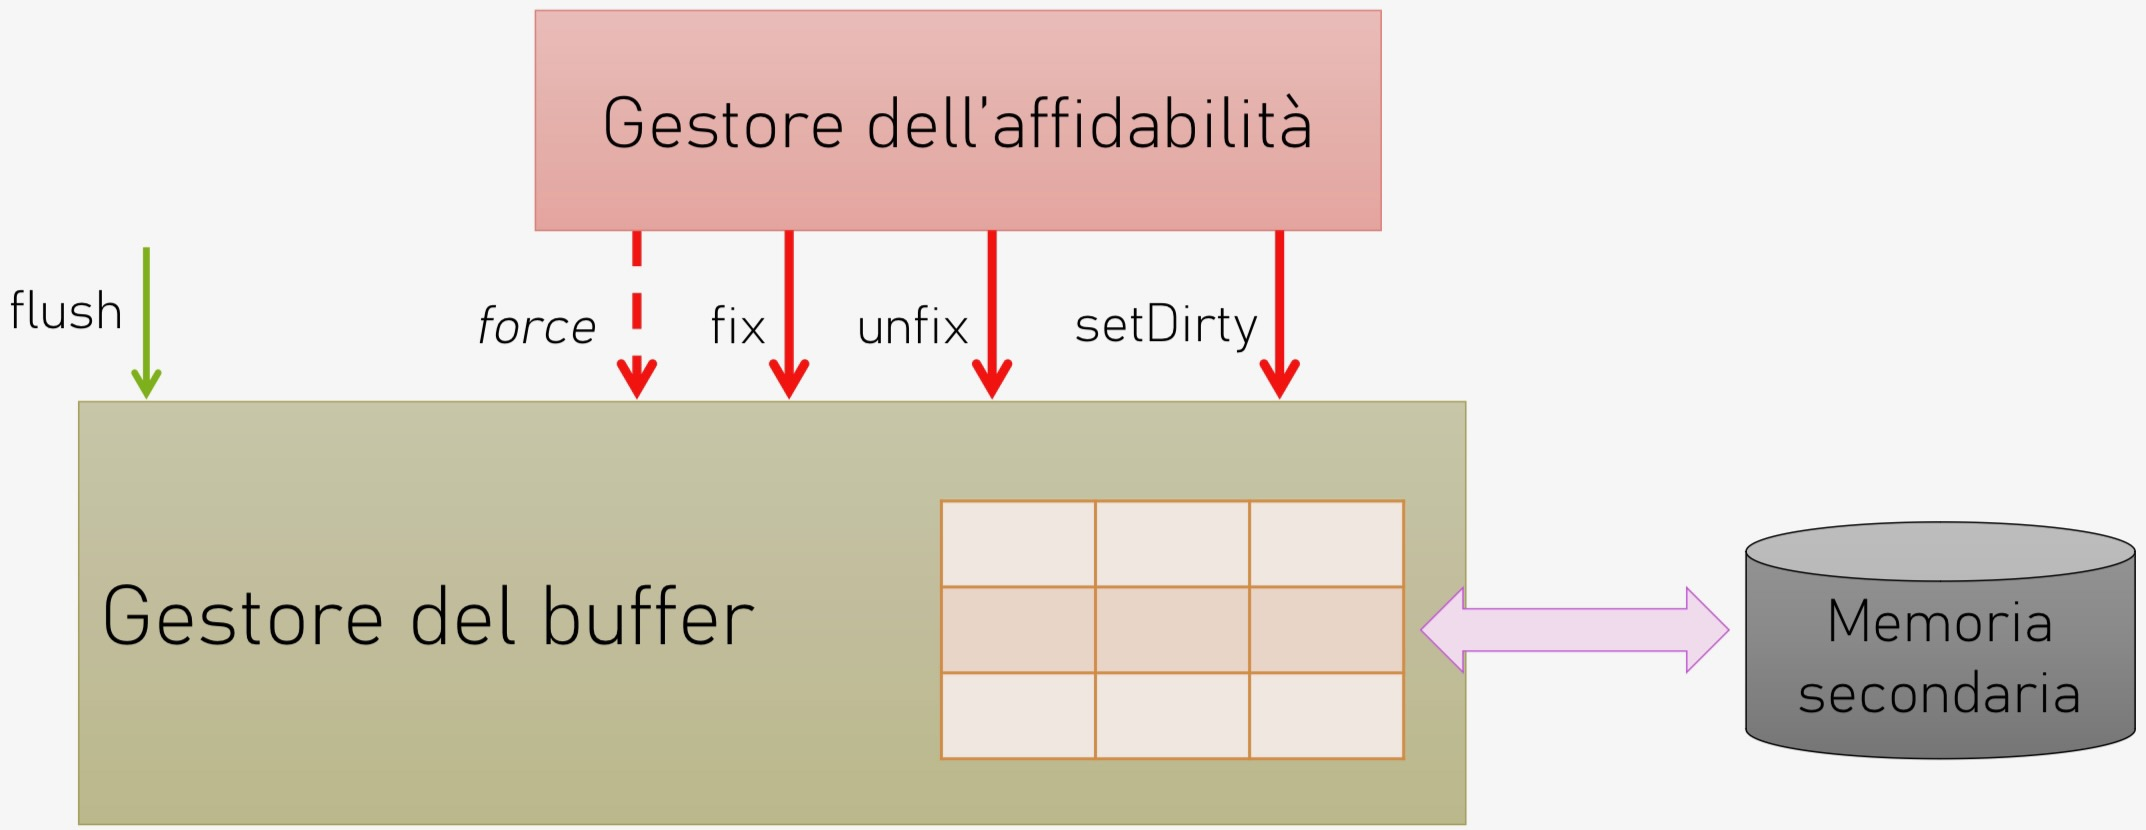
\includegraphics[width=15cm]{img/affidabilita.jpeg}
    \caption{Gestore dell'affidabilità}
    \label{fig:affidabilita}
\end{figure}
È il modulo responsabile di ciò che riguarda l'esecuzione delle istruzioni 
per la gestione delle transazioni e la della realizzazione delle operazioni 
necessarie al ripristino della base di dati dopo eventuali malfunzionamenti.

Per il suo funzionamento il gestore dell'affidabilità deve disporre di un 
dispositivo di memoria stabile, cioè resistente a guasti.
\subsection{Gestione del file di $\texttt{LOG}$}
In memoria stabile viene memorizzato il file di \verb|LOG| che registra in 
modo sequenziale le operazioni eseguite dalle transazioni sulla base 
di dati.
I record memorizzati sul file di \verb|LOG| di suddividono in record di 
transazione e di sistema.

I record di transazione si classificano in:
\begin{itemize}
    \item Begin della transazione $\verb|T|$: $\verb|B(T)|$.
    \item Commit della transazione $\verb|T|$: $\verb|C(T)|$.
    \item Abort della transazione $\verb|T|$: $\verb|A(T)|$.
    \item Insert, Delete e Update eseguiti dalla transazione $\verb|T|$ sull'oggetto $\verb|O|$:
    \begin{itemize}
        \item $\verb|I(T,O,AS)|$: dove $\verb|AS|$ indica After State.
        \item $\verb|D(T,O,BS)|$: dove $\verb|BS|$ indica Before State.
        \item $\verb|U(T,O,BS,AS)|$
    \end{itemize}
\end{itemize}
I record di transazione salvati nel LOG consentono di eseguire,
in caso di ripristino, le seguenti operazioni:
\begin{itemize}
    \item \verb|UNDO|: per disfare un'azione su un oggetto $O$ è sufficiente 
    ricopiare in $O$ il valore $BS$; l'insert/delete viene disfatto 
    cancellando/inserendo $O$.
    \item \verb|REDO|: per rifare un'azione su un oggetto $O$ è sufficiente 
    ricopiare in $O$ il valore $AS$; l'insert/delete viene rifatto 
    cancellando/inserendo $O$.
\end{itemize}
Gli inserimenti controllano sempre l'esistenza di $O$ (\textit{non si 
inseriscono duplicati}).

I record di sistema:
\begin{itemize}
    \item Operazioni di \verb|DUMP| della base di dati: $\texttt{DUMP}$.
    \item Operazioni di \verb|CheckPoint|: $\texttt{CK}(T_1,\dots,T_n)$ indica che l'esecuzione 
    del CheckPoint le transazioni attive erano $T_1, \dots, T_n$.
    \item L'operazione svolta periodicamente dal gestore dell'affidabilità prevede:
    \begin{itemize}
        \item Sospensione delle operazioni di scrittura, commit e abort delle transazioni.
        \item Esecuzione della primitiva force sulle pagine \textit{dirty} di transazioni che hanno eseguito il commit.
        \item Scritture sincrona sul file \verb|LOG| del record di CheckPoint con gli 
        identificatori delle transazioni attive.
        \item Ripresa delle operazioni di scrittura, commit e abort delle transazioni.
    \end{itemize}
\end{itemize}
\subsubsection{Regole di scrittura sul \texttt{LOG}}
\begin{itemize}
    \item Regola WAL (\textit{Write Ahead Log}): i record di log devono 
    essere scritti sul \verb|LOG| prima dell'esecuzione delle corrispondenti operazioni sulla base di dati 
    (\textit{garantisce la possibilità di fare sempre $\texttt{UNDO}$}).
    \item Regola Commit-Precedenza: i record di log devono essere 
    scritti prima dell'esecuzione del commit della transazione (\textit{Garantisce 
    la possibilità di fare $\texttt{REDO}$}).
\end{itemize}
Tali regole consentono inoltre di salvare i blocchi delle pagine "dirty" in 
modo totalmente asincrono rispetto al commit delle transazioni.
\subsubsection{Azione di commit}
Una transazione \verb|T| sceglie in modo atomico l'esito di commit nel momento in cui 
scrive nel file di log in modo sincrono (\textit{primitiva $\texttt{force}$}) il suo record di commit \verb|C(T)|.
\begin{itemize}
    \item Se il guasto avviene prima della scrittura del record di commit $\verb|UNDO|$.
    \item Se il guasto avviene dopo la scrittura del record di commit $\verb|REDO|$.
\end{itemize}
\subsubsection{Gestore dell'affidabilità}
Il gestore dell'affidabilità gestisce due tipologie di guasto:
\begin{itemize}
    \item Guasto di sistema: perdita del contenuto della memoria centrale, gestibile attraverso
    la ripresa a caldo.
    \item Guasto di dispositivo: perdita di parte o tutto il contenuto 
    della base di dati in memoria, gestibile attraverso la ripresa a freddo.
\end{itemize}
\begin{figure}[H]
    \centering
    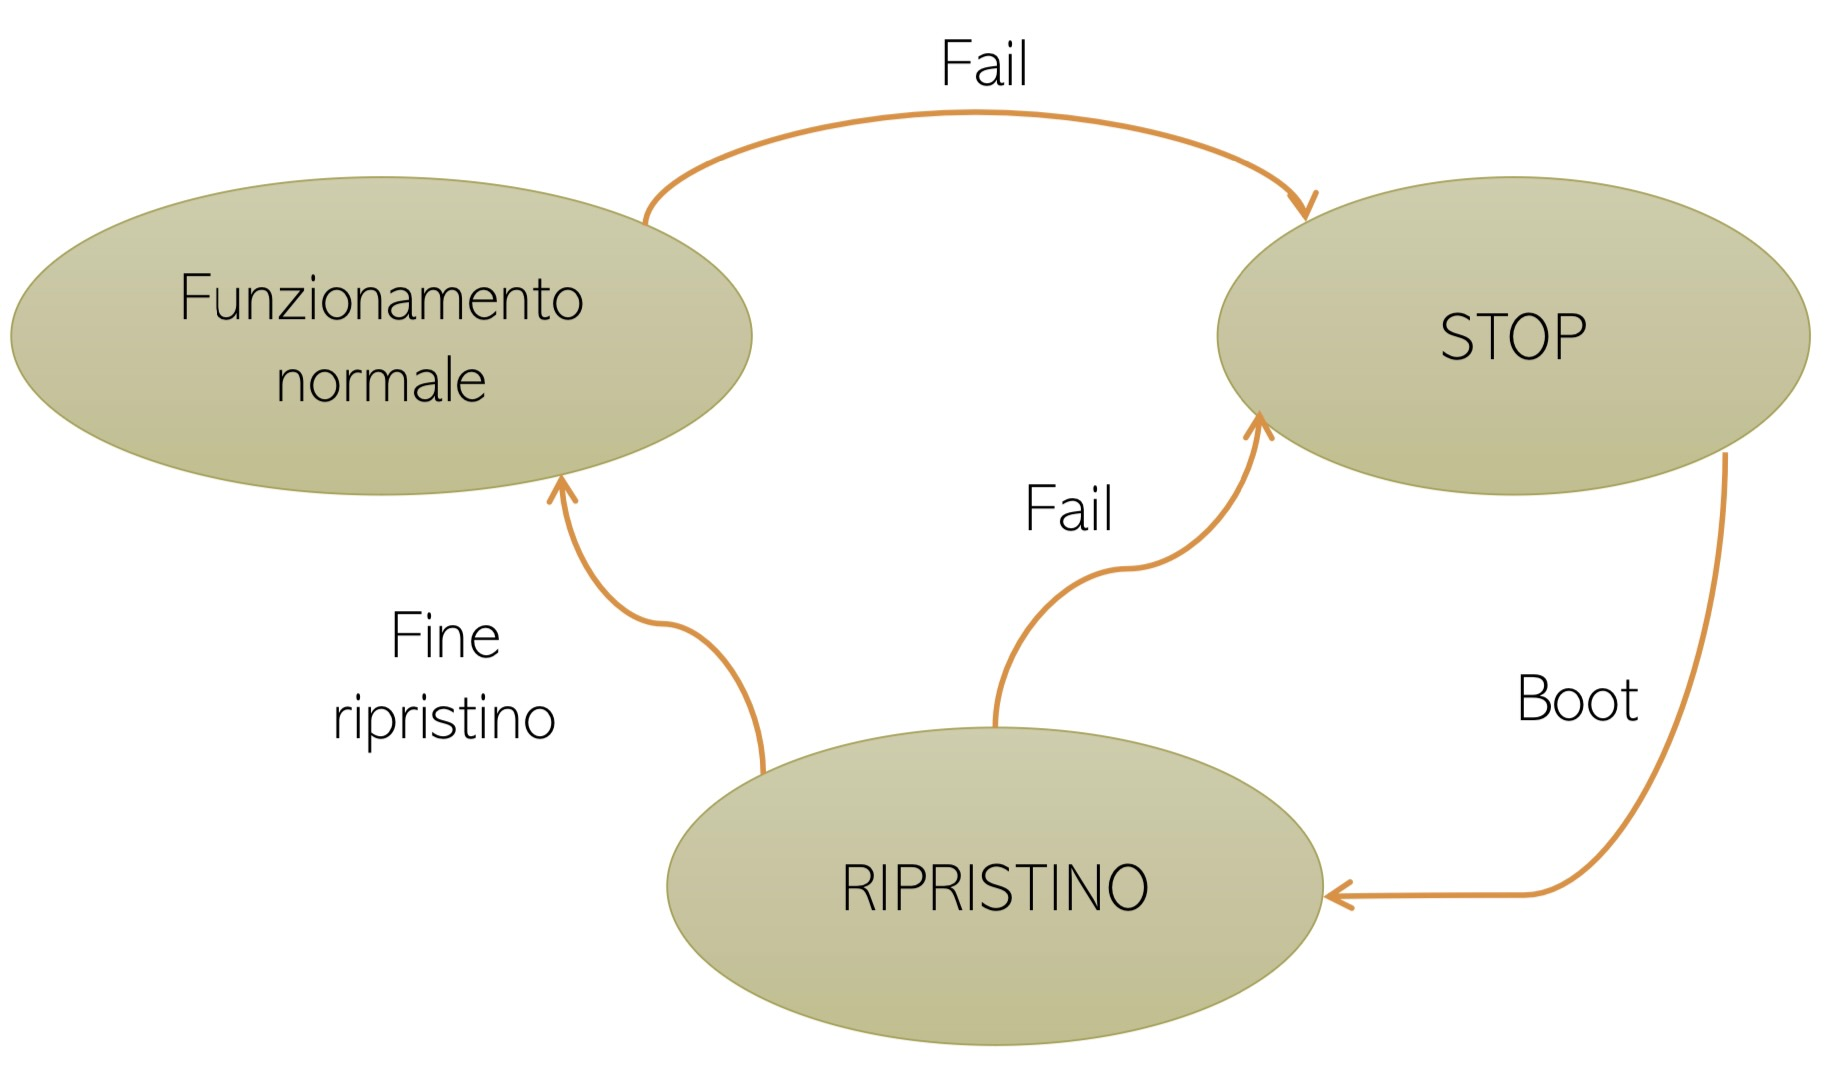
\includegraphics[width=9cm]{img/modelloAffidabilita.jpeg}
    \caption{Modello di funzionamento}
    \label{fig:Modelloaffidabilita}
\end{figure}
\subsection{Ripresa a caldo}
\begin{itemize}
    \item Si accede all'ultimo blocco di \verb|LOG| e si ripercorre all'indietro il \verb|LOG| 
    fino al più recente record \verb|CK|.
    \item Si decidono le transazioni da rifare/disfare inizializzando l'insieme $\verb|UNDO|$ con 
    le transazioni attive al $\verb|CK|$ e l'insieme $\verb|REDO|$ con l'insieme vuoto.
    \item Si ripercorre in avanti il \verb|LOG| e per ogni record $\verb|B(T)|$ incontrato 
    si aggiunge $\verb|T|$ a $\verb|UNDO|$ e per ogni record $\verb|C(T)|$ incontrato si sposta $\verb|T|$ da $\verb|UNDO|$ a $\verb|REDO|$.
    \item Si ripercorre all’indietro il \verb|LOG| disfacendo le operazioni eseguite dalle transazioni in 
    $\verb|UNDO|$ risalendo fino alla prima azione della transazione più vecchia.
    \item Si rifanno le operazioni delle transazioni dell'insieme $\verb|REDO|$.
\end{itemize}
\subsection{Ripresa a freddo}
\begin{itemize}
    \item Si accede al $\verb|DUMP|$ della base di dati e si ricopia selettivamente la 
    parte deteriorata della base di dati.
    \item Si accede al \verb|LOG| risalendo al record $\verb|DUMP|$.
    \item Si ripercorre in avanti il \verb|LOG| rieseguendo tutte le operazioni relative alla parte deteriorata
    comprese le azioni di commit e abort.
    \item Si applica una ripresa a caldo.
\end{itemize}
\chapter{Strutture fisiche e strutture di accesso ai dati}
\section{Gestore dei metodi di accesso}
Il gestore dei metodi d'accesso è un modulo del DBMS che esegue il piano di esecuzione 
prodotto dall'ottimizzatore e produce sequenze di accessi ai blocchi della base di dati 
presenti in memoria secondaria.
\begin{tcolorbox}[title={Metodi d'accesso}]
Sono software che implementano gli algoritmi di accesso e manipolazione dei dati 
organizzati in specifiche strutture fisiche.
\end{tcolorbox}
Ogni metodo d'accesso ai dati conosce:
\begin{itemize}
    \item L'organizzazione delle tuple/record di indice nei blocchi \verb|DATI/INDICE| salvati
    in memoria secondaria (\textit{come una tabella/indice viene organizzata 
    in blocchi $\texttt{DATI}$ della memoria secondaria});
    \item L’organizzazione fisica interna dei blocchi sia quando contengono \verb|DATI| 
    (\textit{vale a dire, tuple di una tabella}) sia quando contengono strutture 
    fisiche di accesso o \verb|INDICI| (\textit{vale a dire, record di un indice}).
\end{itemize}
\subsection{Organizzazione di un blocco DATI}
In un blocco \verb|DATI| sono presenti informazioni utili e informazioni di controllo:
\begin{itemize}
    \item Informazioni utili: tuple della tabella;
    \item Informazioni di controllo: dizionario, bit di parità, altre informazioni del 
    file system o della specifica struttura fisiche.
\end{itemize}
\begin{figure}[H]
    \centering
    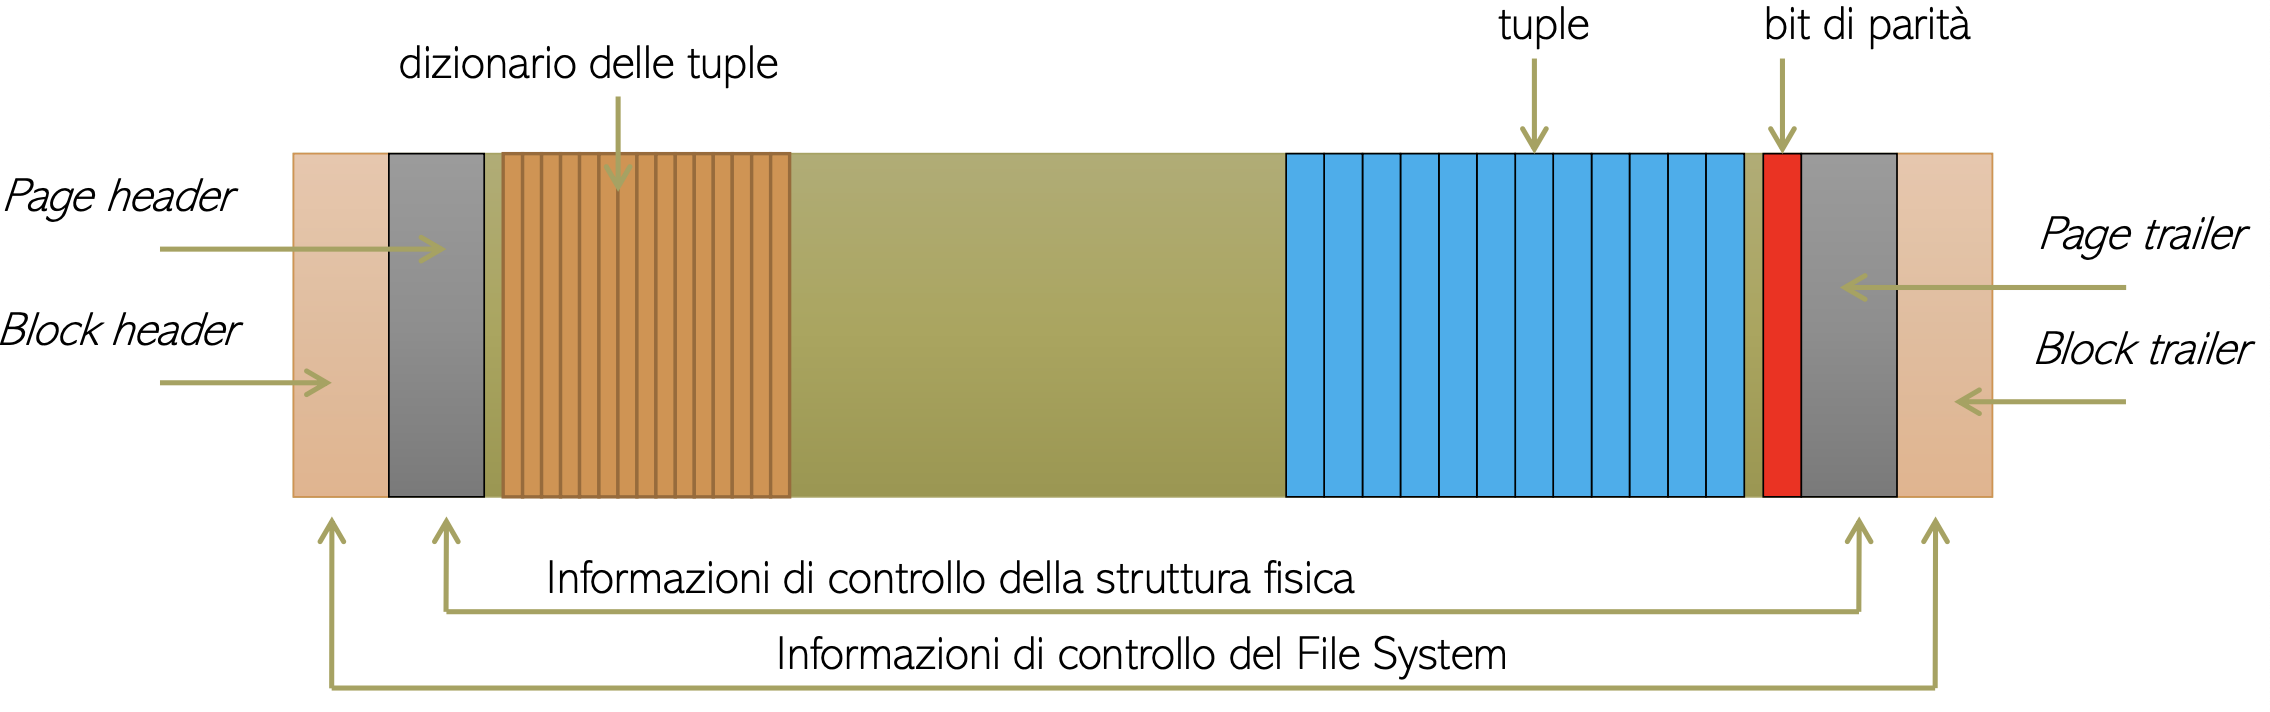
\includegraphics[width=15cm]{img/Tabella_livello_fisico.png}
    \caption{Struttura della pagina}
    \label{fig:pagina_struttura}
\end{figure}
\subsection{Struttura del dizionario}
Vi sono due opzioni:
\begin{itemize}
    \item Tuple di \textbf{lunghezza fissa}: il dizionario non è necessario, 
    si deve solo memorizzare la dimensione delle tuple e l'offset del punto iniziale.
    \item Tuple di \textbf{lunghezza variabile}: il dizionario memorizza l'offset di ogni 
    tuple presente nel blocco e di ogni attributo di ogni tupla.
\end{itemize}
La lunghezza massima della tupla è pari alla dimensione massima dell'area disponibile su un blocco,
altrimenti va gestito il caso di tuple memorizzate su più blocchi.
\subsection{Operazioni sulle pagine}
\begin{itemize}
    \item Inserimento di una tupla:
    \begin{itemize}
        \item Se esiste spazio contiguo sufficiente: inserimento semplice;
        \item Se non esiste spazio contiguo, ma esiste spazio sufficiente: riorganizza 
        lo spazio ed esegue un inserimento semplice;
        \item Se non esiste spazio sufficiente: operazione rifiutata.
    \end{itemize}
    \item Cancellazione: sempre possibile anche senza riorganizzare;
    \item Accesso ad una tupla;
    \item Accesso ad un attributo di una tupla;
    \item Accesso sequenziale (\textit{di solito in orine di chiave primaria});
    \item Riorganizzare.
\end{itemize}
\begin{figure}[H]
    \centering
    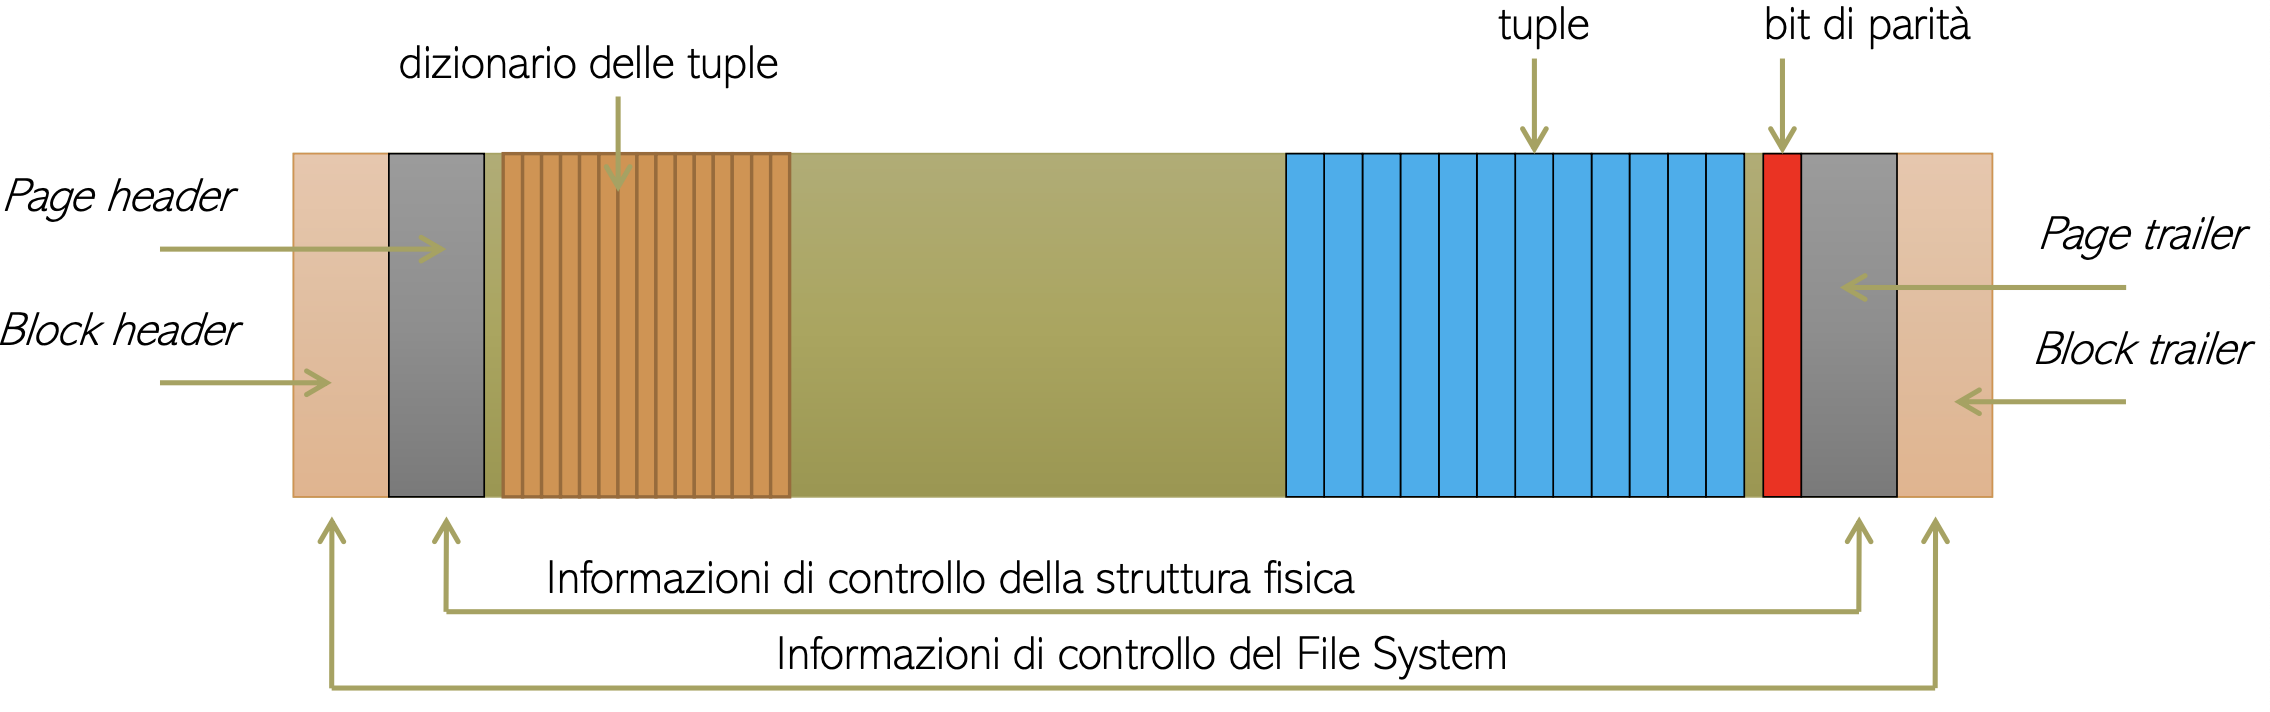
\includegraphics[width=15cm]{img/Tabella_livello_fisico.png}
    \caption{Rappresentazione di tabella a livello fisico}
    \label{fig:tab_liv_fis}
\end{figure}
\section{Struttura sequenziale ordinata}
Una struttura sequenziale ordinata è un \textbf{file sequenziale}  dove 
le tuple sono ordinate secondo \textbf{chiave di ordinamento}.
\subsubsection{Esempio}
\begin{figure}[H]
    \centering
    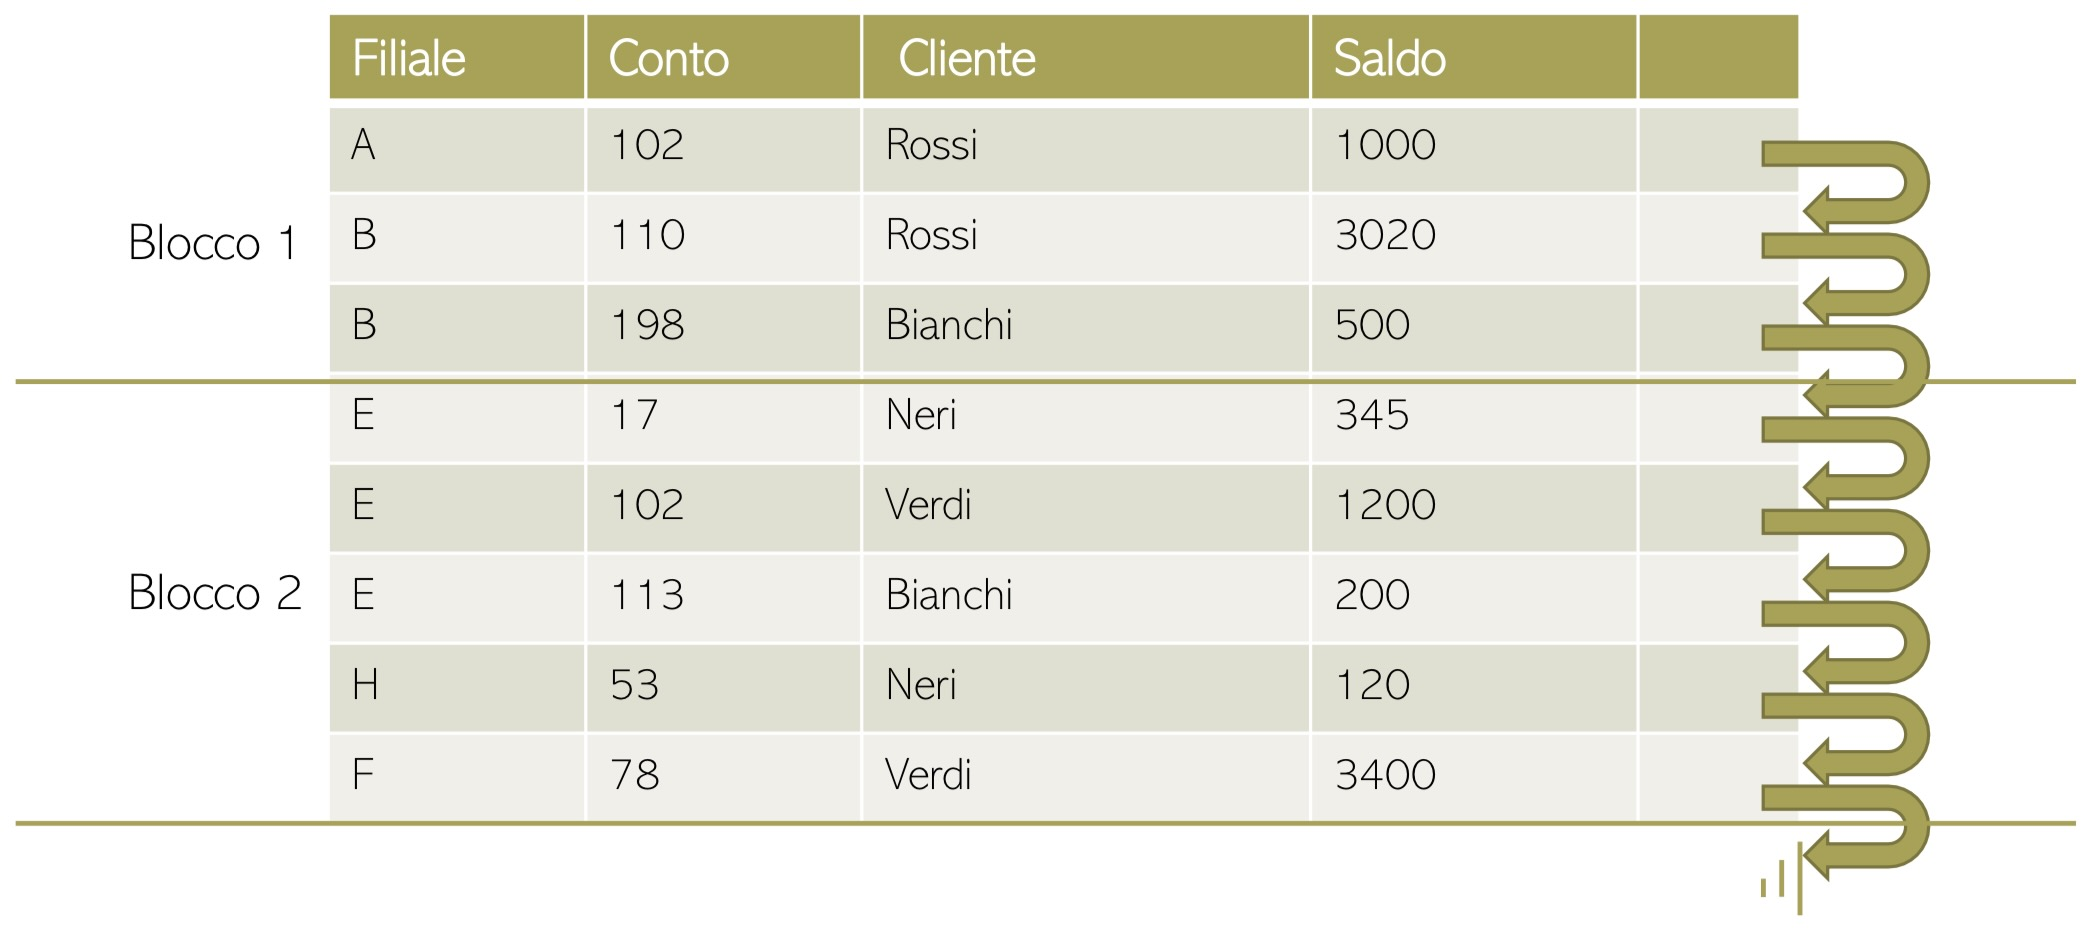
\includegraphics[width=9cm]{img/esempio_index.jpeg}
    \caption{Esempio}
    \label{fig:Es_index}
\end{figure}
\subsection{Operazioni}
L'inserimento di una tupla avviene seguendo i seguenti passi:
\begin{itemize}
    \item Individuazione del blocco che \textbf{contiene la tupla che precede},
    nell'ordine della chiave, la tupla da inserire.
    \item Inserimento della tupla nuova in $B$; se l'operazione non va a buon fine 
    si aggiunge un nuovo blocco (\textit{detto, overflow page}) alla struttura: 
    il blocco contiene la nuova tupla, altrimenti si prosegue.
    \item Aggiustamento della catena di puntatori.
\end{itemize}

La scansione sequenziale ordinata avviene secondo la chiave (\textit{seguendo 
i puntatori}).

La cancellazione di una tupla avviene seguendo i seguenti passi:
\begin{itemize}
    \item Individuazione del blocco $\verb|B|$ che contiene la tupla da cancellare.
    \item Cancellazione della tupla $\verb|B|$.
    \item Aggiustamento della catena di puntatori.
\end{itemize}

La riorganizzazione avviene assegnando le tuple ai blocchi ed opportuni coefficienti 
di riempimento, riaggiustando i puntatori.
\section{Indici}
Per aumentare le prestazioni degli accessi alle tuple memorizzate nelle strutture fisiche 
(\textbf{file sequenziale}), si introducono strutture ausiliarie (\textit{dette 
strutture ai dati o indici}); tali strutture velocizzano l'accesso casuale via chiave di ricerca.
La chiave di ricerca è un insieme di attributi utilizzati dall'indice nella ricerca.

Gli indici su file sequenziali possono essere di due categorie:
\begin{itemize}
    \item \textbf{Indice primario}: in questo caso la \textbf{chiave di ordinamento} del file 
    sequenziale coincide con la \textbf{con la chiave di ricerca} dell'indice.
    \item \textbf{Indice secondario}: in questo caso invece la \textbf{chiave di 
    ordinamento} e la \textbf{chiave di ricerca} sono \textbf{diverse}.
\end{itemize}
\subsection{Indice primario}
L'indice primario usa una \textbf{chiave di ricerca} che coincide con la chiave di 
ordinamento del file sequenziale.

Ogni record dell'indice primario contiene una coppia $\langle v_i, p_i\rangle$ dove:
\begin{itemize}
    \item $v_i$: valore della chiave di ricerca.
    \item $p_i$: puntatore al primo record del file sequenziale con chiave $v_i$.
\end{itemize}
Esistono due varianti dell'indice primario:
\begin{itemize}
    \item Indice denso: per ogni occorrenza della chiave presente nel file esiste 
    un corrispondente record nell'indice.
    \item Indice sparso: solo per alcune occorrenze della chiave presente nel file 
    esiste un corrispondente record nell'indice, tipicamente una per blocco.
\end{itemize}
\subsubsection{Operazioni di ricerca}
La ricerca di una tupla con chive di ricerca $K$ si differenzia per le due 
modalità:
\begin{itemize}
    \item Denso: in questo caso $K$ è presente nell'indice e si esegue una scansione 
    sequenziale dell'indice per trovare il record $(K, p_k)$ e si accede al file 
    attraverso puntatore $p_k$. Il costo dell'operazione è di un accesso all'indice più 
    un accesso al blocco dati.
    \item Sparso: in questo caso $k$ potrebbe non essere presente nell'indice e si 
    esegue una scansione sequenziale dell'indice fino al record $(K',p'_k)$ dove $k'$ 
    è il valore più grande che sia minore o uguale a $K$. Si esegue un accesso attraverso 
    il puntatore $p_k'$ e si scansiona il file (\textit{blocco corrente}) per trovare 
    le tuple con chiave $K$. Il costo dell'operazione è di un accesso all'indice più 
    un accesso al blocco dati.
\end{itemize}
\subsubsection{Operazioni di inserimento}
L'inserimento nel file sequenziale si differenzia per le due modalità:
\begin{itemize}
    \item Denso: l'inserimento nell'indice avviene solo se la tupla inserita nel file ha
    un valore di chiave $K$ che non è già presente.
    \item Sparso: l'inserimento avviene solo quando, per effetto dell'inserimento di 
    una nuova tupla, si aggiunge un blocco dati alla struttura; in tutti gli altri 
    casi l'indice rimane invariato.
\end{itemize}
\subsubsection{Operazioni di cancellazione}
La cancellazione di un record nell'indice si differenzia per le due modalità:
\begin{itemize}
    \item Denso: la cancellazione nell'indice avviene solo se la tupla cancellata 
    nel file è l'ultima tupla con valore di chiave $K$.
    \item Sparso: la cancellazione nell'indice avviene solo quando $K$ è presente 
    nell'indice e il corrispondente blocco viene eliminato; altrimenti, se il 
    blocco sopravvive, va sostituito $K$ nel record dell'indice con il primo valore 
    $K'$ presente nel blocco.
\end{itemize}
\subsection{Indice secondario}
L'indice secondario una una chiave che non coincide con la chiave di ordinamento del file 
sequenziale. Ogni record dell'indice secondario contiene una coppia $\langle v_i,p_i\rangle$:
\begin{itemize}
    \item $v_i$: valore nella chiave di ricerca.
    \item $p_i$: puntatore al bucket di puntatori che individuano nel file 
    sequenziale tutte le tuple con valore di chiave $v_i$.
\end{itemize}
A differenzia degli indici primari, gli indici secondari sono sempre densi.
\subsection{Operazioni di ricerca}
L'operazione di ricerca di una tupla con chiave di ricerca $K$ avviene eseguendo 
una scansione sequenziale dell'indice per trovare il record $(K,p_k)$, viene eseguito 
l'accesso al bucket di puntatori attraverso il puntatore $p_k$ e successivamente un accesso al file 
attraverso i puntatori del bucket $B$.

Il costo dell'operazione è di un accesso all'indice più l'accesso al bucket e più 
gli $n$ accessi alle pagine dati.
\subsubsection{Operazioni di inserimento e cancellazione}
Tali operazioni vengono eseguite come per l'indice primario denso con più 
l'aggiornamento dei bucket.
\section{B+-Tree} 
Quando l'indice aumenta di dimensioni, non può risiedere in memoria centrale: di conseguenza
deve essere in grado di essere gestito in memoria secondaria. È possibile utilizzare 
un \textbf{file sequenziale ordinato} per rappresentare l'\textbf{indice in memoria 
secondaria}, le prestazioni di accesso a tale struttura fisica a fronte di inserimenti/cancellazioni 
tendono a denigrare e richiedono frequenti riorganizzazioni. Inoltre è disponibile solo 
l'accesso sequenziale.

Per superare tale problema si introducono per gli indici strutture fisiche diverse, tra cui 
\textbf{strutture ad albero} e le \textbf{strutture ad accesso calcolato}.

Nel B+-tree ogni nodo corrisponde ad una pagina della memoria secondaria e i legami tra nodi 
diventano puntatori a pagina. Ogni nodo ha un numero elevato di figli, quindi l'albero ha tipicamente 
\textbf{pochi livelli e molti nodi foglia}.

L'albero è inoltre bilanciato, ciò significa che la lunghezza dei percorsi che collegano 
la radice ai nodi foglia è costante, inoltre gli inserimenti e le cancellazioni 
non alterano le prestazioni dell'accesso ai dati: l'albero si mantiene bilanciato.

\subsection{Struttura}
La struttura di un B+-tree può contenere fino a $n-1$ valori 
ordinati di chiave di ricerca e fino a $n$ puntatori.

Il puntatore $p_m$ del nodo al livello superiore $L_i$ punta al nodo del livello inferiore 
$L_{i+1}$ se esiste.
\begin{figure}[H]
  \begin{center}
    \scalebox{0.8}{
     \begin{tikzpicture}
        % 
        \btreeinodefour{root}{$K_1$}{$K_2$}{\dots}{$K_{m+1}$};
        \xyshift{10mm}{-20mm}{\btreeinodefour{n1}{$K_1'$}{$K_2'$}{\dots}{$K_{m-1}'$}};
        %\foreach \x in {1,2,...,4} { \btreelink{root-\x}{n\x}}
        \btreelink{root-5}{n1}
      \end{tikzpicture}
    }
  \end{center}
\end{figure}
Se un puntatore è compreso tra i valori $K_{i-1}$ e $K_i$ 
tale puntatore punterà al sottoalbero con chiavi $k$ tali che:
$K_{i-1}<k<K_i$
\subsection{Vincoli di riempimento}
Ogni nodo foglia contiene un numero di valori chiave ($\#chiavi$) 
vincolato come segue:
\[
  \left\lceil \frac{n-1}{2}\right\rceil \leq \#chiavi \leq n-1
\]
Ogni nodo intermedio contiene un numero di puntatori ($\#puntatori$) 
vincolato come segue (\textit{per la radice non vale il minimo}):
\[
  \left\lceil \frac{n}{2}\right\rceil \leq \#puntatori \leq n
\]
\subsubsection{Esempio fan-out 4}
\begin{figure}[H]
  \begin{center}
    \scalebox{0.7}{
     \begin{tikzpicture}
        % 
        \btreeinodeone{root}{R};
        \xyshift{-40mm}{-20mm}{\btreeinodetwo{n1}{L}{P}};
        \xyshift{40mm}{-20mm}{\btreeinodeone{n2}{X}};
        \xyshift{-90mm}{-40mm}{\btreeinodefour{m1}{A}{B}{C}{D}};
        \xyshift{-40mm}{-40mm}{\btreeinodefour{m2}{L}{M}{N}{O}};
        \xyshift{0mm}{-40mm}{\btreeinodetwo{m3}{P}{Q}};
        \xyshift{40mm}{-40mm}{\btreeinodefour{m4}{R}{S}{T}{V}};
        \xyshift{80mm}{-40mm}{\btreeinodetwo{m5}{X}{Z}};
        \btreelinknorth{root}{n1}
        \btreelinknorth{root}{n2}
        \foreach \x in {1,2,...,3} { \btreelink{n1-\x}{m\x}}
        \btreelink{n2-1}{m4}
        \btreelink{n2-2}{m5}
      \end{tikzpicture}
    }
  \end{center}
\end{figure}
\subsection{Operazioni}
\subsubsection{Ricerca}
La ricerca si effettua attraverso diversi passi:
\begin{enumerate}
  \item Cercare nel nodo radice il più piccolo valore di 
  chiave maggiore di $\verb|K|$.
  \begin{itemize}
    \item Se esiste allora si segue il puntatore $p_i$.
    \item Se tale valore non esiste si segue il puntatore $p_m$.
  \end{itemize}
  \item Se il nodo raggiunto è un nodo foglia cercare il valore 
  $\verb|K|$ nel nodo e seguire il corrisponde puntatore verso le tuple, 
  altrimenti riprendere il passo $(1)$.
\end{enumerate}
\subsubsection{Inserimento con chiave $\texttt{K}$}
\begin{enumerate}
  \item Ricerca del nodo foglia $\verb|NF|$ dove il valore $\verb|K|$ va inserito
  \item Se $\verb|K|$ è presente in $\verb|NF|$, allora:
  \begin{itemize}
    \item Indice primario: nessuna azione;
    \item Indice secondario: aggiornamento del bucket di puntatori.
  \end{itemize}
  Altrimenti, inserire $\verb|K|$ in $\verb|NF|$ rispettando l'ordine e:
  \begin{itemize}
    \item Indice primario: inserire il puntatore alla tupla con valore $K$ 
    della chiave;
    \item Indice secondario: inserire un nuovo bucket di puntatori contenente 
    il puntatore alla tupla con valore $\verb|K|$ della chiave.
  \end{itemize}
\end{enumerate}
Se non è possibile inserire $\verb|K|$ in $\verb|NF|$, allora si esegue uno split di $\verb|NF|$.

Nel nodo da dividere esistono $n$ valori chiave, si procede come segue:
\begin{itemize}
  \item Creare due nodi foglia;
  \item Inserire i primi $\lceil (n-1)/2\rceil$ valori nel primo;
  \item Inserire i rimanenti nel secondo;
  \item Inserire nel nodo padre un nuovo puntatore per il secondo nodo 
  foglia generato e riaggiustare i valori chiave presenti nel nodo padre.
  \item Se anche il nodo padre è pieno lo spit si propaga al padre e così via.
\end{itemize}
\subsubsection{Cancellazione con chiave $\texttt{K}$}
\begin{enumerate}
  \item Ricerca del nodo foglia $\verb|NF|$ dove il valore $\verb|K|$ va cancellato.
  \item Cancellare $\verb|K|$ da $\verb|NF|$ insieme al suo puntatore:
  \begin{itemize}
    \item Indice primario: nessuna ulteriore azione;
    \item Indice secondario: liberare il bucket di puntatori.
  \end{itemize}
\end{enumerate}
Se dopo la cancellazione di $\verb|K|$ da $\verb|NF|$ viene violato allora si esegue un merge di $\verb|NF|$.
\section{Hash}
Le caratteristiche generali delle strutture ad accesso calcolato:
\begin{itemize}
  \item Si basano su una funzione di hash che mappa i valori della chiave di ricerca 
  sugli indirizzi di memorizzazione delle tuple nelle pagine dei dati della 
  memoria secondaria.
\end{itemize}
Uso pratico di una funzione di hash negli indici 
\begin{itemize}
  \item Si stima il numero di valori chiave che saranno contenuti nella tabella.
  \item Si alloca un numero di bucket ($\mathcal{B}$) di puntatori uguale al numero stimato.
  \item Si definisce una funzione di folding che trasforma i valori chiave in 
  numeri interi positivi ($\mathbb{K}\rightarrow\mathbb{Z}^+$).
  \item Si definisce una funzione di hashing ($\mathbb{Z}^+\rightarrow\mathcal{B}$).
\end{itemize}
La funzione di hashing distribuisce in modo uniforme e casuale i valori della 
chiave nei bucket. È pesante cambiare la funzione di hashing dopo che la struttura 
d'accesso è stata riempita; si deve costruire l'indice da capo.
\subsection{Operazioni}
\subsubsection{Ricerca}
Dato un valore di chiave $\mathcal{K}$ trovare la corrispondente tupla:
\begin{itemize}
  \item Calcolare $b = h(f({K}))$ (\textit{costo zero});
  \item Accedere al bucket $b$ (\textit{costo: 1 accesso a pagina});
  \item Accedere a $n$ tuple attraverso i puntatori del bucket (\textit{costo: 
  $m$ accessi a pagina $m \leq n$}).
\end{itemize}
\subsubsection{Inserimento e cancellazione}
Di complessità simile alla ricerca.
\subsection{Osservazioni}
La struttura ad accesso calcolato funziona se i buckets conservano un basso coefficiente 
di riempimento. Infatti il problema delle strutture ad accesso calcolato è la 
gestione delle collisioni.

La collisione si verifica quando, dati due valori di chiave $\texttt{K}_1$ e $\texttt{K}_2$, con 
$\texttt{K}_1 \neq \texttt{K}_2$, risulta
\[
  h(f(\texttt{K}_1)) = h(f(\texttt{K}_2))
\]
Un numero eccessivo di collisioni porta alla saturazione del bucket corrispondente.
\subsection{Collisioni}
La probabilità che un bucket riceva $t$ chiavi su $n$ inserimenti:
\[
  p(t) = \binom{n}{t}\left( \frac{1}{B} \right) ^t \left( 1 - \frac{1}{B}\right)^{(n-t)}
\]
Dove B è il numero totale di buckets.

La probabilità di avere più di F collisioni, dove $F$ è il numero di puntatori 
nel bucket è:
\[
  p_k = 1 - \sum_{i=0}^{F}p(i)
\]
\subsection{Gestione delle collisioni}
Un numero eccessivo di collisioni sullo stesso indirizzo porta alla saturazione del bucket corrispondente. Per gestire tale situazione 
si prevede la possibilità di allocare buckets di overflow, collegati di base:
\begin{figure}[H]
  \centering
  \begin{tikzpicture}[%scale=.2,
    node distance = 7mm and 4mm,
      start chain = going right, 
       arr/.style = {semithick, -Stealth},
       dot/.style = {circle, fill, inner sep=1.2pt,
                     label=left:#1},
    every label/.append style = {font=\footnotesize, fill=white, align=center,
                                 fill opacity=0.5, text opacity=1, 
                                 inner sep=1pt},
         E/.style = {ellipse, draw, fill=#1},
      mpnh/.style = {rectangle split, rectangle split horizontal, 
                     rectangle split parts=3, draw, fill=gray!20,
                     inner sep=2pt,
                     on chain},
      mpnv/.style = {rectangle split, rectangle split parts=10,
         rectangle split part fill={gray!30,gray!10,gray!30,gray!30,gray!30,
                                    gray!10,gray!30,gray!10,gray!10,gray!30},
         draw, minimum height=2ex},
       sym/.style = {yshift=-1mm},
       syp/.style = {yshift=+1mm},
                            ]
    \node[mpnv, label=H] (H) 
        {\nodepart{one}     $\diagup$
         \nodepart{two}     \vphantom{$\diagup$} 
         \nodepart{three}   $\diagup$
         \nodepart{four}    $\diagup$
         \nodepart{five}    $\diagup$
         \nodepart{six}     \vphantom{$\diagup$} 
         \nodepart{seven}   $\diagup$
         \nodepart{eight}   \vphantom{$\diagup$} 
         \nodepart{nine}    \vphantom{$\diagup$} 
         \nodepart{ten}     $\diagup$
        };
    %
    \node[mpnh, right=of H.two east] (A1) 
       {\nodepart{one}  $\diagup$
        \nodepart{two}  $k_1$
        \nodepart{three}    \hphantom{$\diagup$}  
       };
    \node[mpnh] (A2)
       {\nodepart{one}      \hphantom{$\diagup$}
        \nodepart{two}      $k_4$
        \nodepart{three}    $\diagup$
       };
    %
    \node[mpnh, right=of H.six east] (B1)
       {\nodepart{one}      $\diagup$
        \nodepart{two}      $k_5$
        \nodepart{three}    \hphantom{$\diagup$}
       };
    \node[mpnh] (B2)
       {\nodepart{one}      \hphantom{$\diagup$}
        \nodepart{two}      $k_2$
        \nodepart{three}    \hphantom{$\diagup$}
       };
    \node[mpnh] (B3)
       {\nodepart{one}      \hphantom{$\diagup$}
        \nodepart{two}      $k_7$
        \nodepart{three}    $\diagup$ 
       };
    %
    \node[mpnh, right=of H.eight east] (C1)
       {\nodepart{one}      $\diagup$
        \nodepart{two}      $k_3$
        \nodepart{three}    $\diagup$
       };
    %
    \node[mpnh, right=of H.nine east] (D1)
       {\nodepart{one}  $\diagup$
        \nodepart{two}  $k_8$
        \nodepart{three}    \hphantom{$\diagup$}
       };
    \node[mpnh] (D2)
       {\nodepart{one}      \hphantom{$\diagup$}
        \nodepart{two}      $k_6$
        \nodepart{three}    $\diagup$
       };
    %% arrows (right)
    \draw[arr]  (H |- H.two east)   edge (A1)
                (H |- H.six east)   edge (B1)
                (H |- H.eight east) edge (C1)
                (H |- H.nine east)   to (D1)
                ;
    \draw[arr, transform canvas={yshift=1mm}]  
                (A1.three north |- A1.east)  edge (A2)
                (B1.three north |- B1.east)  edge (B2)
                (B2.three north |- B2.east)  edge (B3)
                (D1.three north |- D2)   to   (D2)
                ;
    \draw[arr, transform canvas={yshift=-1mm}]
                (A2.one north |- A2)  edge  (A1)
                (B2.one north |- B2)  edge  (B1)
                (B3.one north |- B3)  edge  (B2)
                (D2.one north |- D2)   to   (D1)
                ;
        \end{tikzpicture}
\end{figure}
\section{Confronto tra B+-tree e Hashing}
Per quanto riguarda la ricerca con selezioni basate su uguaglianza , ovvero $A = cost$,
l'hashing (senza overflow buckets) è a tempo costante, mentre il B+-tree è a tempo 
logaritmico nel numero di chiavi.

Le selezioni basate su intervalli (\textit{range}), l'hashing: ha un numero 
elevato di selezioni su condizioni si uguaglianza per scandire tutti i valori del range, mentre 
il B+-tree è a tempo logaritmico per accedere al primo valore dell'intervallo, 
scandendo i nodi foglia fino all'ultimo valore compreso.

Gli inserimenti e le cancellazioni nell'hashing sono a tempo costante, più l'eventuale 
gestione dell'overflow, mentre per il B+-tree sono a tempo logaritmico nel numero di chiavi, 
più eventuali split e merge.
\chapter{Esecuzione concorrente di transazioni}
Per gestire con prestazioni accettabili il carico di lavoro tipico delle applicazioni 
gestionali, un DBMS deve eseguire le transazioni in modo concorrente.
L'esecuzione concorrente di transazioni senza controllo può generare anomalie 
o problemi di correttezza. È quindi necessario introdurre dei meccanismi di controllo 
nell'esecuzione delle transazioni per evitare tali anomalie.
\section{Anomalie di esecuzione concorrente}
Le anomalie tipiche sono:
\begin{itemize}
  \item Perdita di aggiornamento (\textit{update}): gli effetti di una transazione 
  concorrente sono persi.
  \item Lettura inconsistente: accessi successivi ad uno stesso dato all'interno 
  di una transazione ritornano valori diversi.
  \item Lettura sporca: viene letto un dato che rappresenta uno stato intermedio
  nell'evoluzione di una transazione.
  \item Aggiornamento/inserimento fantasma: valutazioni diverse di valori aggregati 
  a causa di inserimenti intermedi.
\end{itemize}

\subsubsection{Notazione}
\begin{itemize}
  \item Indicheremo con $t_i$ una transazione.
  \item $r_i(x)$: è un'operazione di lettura eseguita dalle transazioni 
  $t_i$ sulla risorsa $x$.
  \item $w_i(x)$: è un'operazione di scrittura eseguita dalle transazioni 
  $t_i$ sulla risorsa $x$.
\end{itemize}
\section{Schedule}
Lo schedule è una sequenza di istruzioni di lettura e scrittura eseguite su 
risorse della base di dati da diverse transazioni concorrenti.
\[
  \mathcal{S}:r_1(x)r_2(z)w_1(x)w_2(z)
\]
Esso rappresenta una possibile esecuzione concorrente di diverse transazioni.
\subsection{Schedule seriale}
Lo schedule seriale è uno schedule dove le operazioni di ogni transazione compaiono 
in sequenza \textbf{senza essere inframezzate} da operazioni di altre transazioni.
\[
  \mathcal{S}_1:r_1(x)r_2(x)w_2(x)w_1(x)\qquad \textit{Non è seriale}
\]
\[
  \mathcal{S}_2:r_1(x)w_1(x)r_2(x)w_2(x)\qquad \textit{È seriale}
\]
\subsection{Schedule serializzabile}
Lo schedule serializzabile è uno schedule equivalente ad uno schedule seriale.

A questo punto occorre definire il concetto di \textbf{equivalenza} tra schedule.
\begin{tcolorbox}[title = {Equivalenza}]
L'idea è che si vogliono considerare equivalenti due schedule che \textbf{producono gli stessi 
effetti sulla base di dati}. Quindi accettare schedule serializzabili significa 
accettare schedule che hanno gli stessi effetti di uno schedule seriale.
\end{tcolorbox}
\section{Equivalenza tra schedule}
\subsection{Ipotesi di commit-proiezione}
Si suppone che le transazioni abbiano esito noto. Quindi si tolgono dagli schedule 
tutte le operazioni delle transazioni che non vanno a buon fine.

Richiedono questa ipotesi le seguenti tecniche di gestione della concorrenza:
\begin{itemize}
  \item Gestione della concorrenza basata sulla \textbf{view-equivalenza}
  \item Gestione della concorrenza basata sulla \textbf{conflict-equivalenza}.
\end{itemize}
\subsubsection{View-equivalenza}
Prima di definire la view-equivalenza vediamo delle definizioni preliminari.

\begin{tcolorbox}[title = {Legge da}]
Dato uno schema $\mathcal{S}$ si dice che un'operazione di lettura $r_i(x)$ che compare in $\mathcal{S}$,
fa parte dell'insieme \verb|LEGGE_DA|, se $w_j(x)$ precede $r_i(x)$ in $\mathcal{S}$
e non vi è alcuna operazione $w_k(x)$ tra le due.
\end{tcolorbox}
\subsubsection{Esempio}
\[
  \mathcal{S}_1:r_1(x)r_2(x)w_2(x)w_1(x)\qquad\verb|LEGGE_DA|(\mathcal{S}_1)=\varnothing
\]
\[
  \mathcal{S}_1:w_1(x)r_2(x)w_2(x)w_1(x)\qquad\verb|LEGGE_DA|(\mathcal{S}_1)=\{(r_2(x),w_1(x))\}
\]

\begin{tcolorbox}[title = {Scritture finali}]
  Dato uno schema $\mathcal{S}$ si dice che un'operazione di scrittura $w_i(x)$,
  che compare in $\mathcal{S}$, appartiene all'insieme \verb|SCRITTURE_FINALI| se è l'ultima operazione di scrittura della risorsa $x$
  in $\mathcal{S}$.
  \end{tcolorbox}
  \subsubsection{Esempio}
  \[
    \mathcal{S}_1:r_1(x)r_2(x)w_2(x)w_2(y)w_1(x)\qquad\verb|SCRITTURE_FINALI|(\mathcal{S}_1)=\{w_3(y),w_1(x)\}
  \]
  \[
    \mathcal{S}_1:r1(x)w_1(x)r_2(x)w_2(x)w_3(y)\qquad\verb|SCRITTURE_FINALI|(\mathcal{S}_1)=\{(w_2(x),w_3(y))\}
  \]

\begin{tcolorbox}[title = {View-equivalenza}]
  Da schedule $S_1$ e $S_2$ sono view-equivalenti ($\mathcal{S}_1 \approx_V \mathcal{S}_2$) se 
  possiedono le stesse relazioni \verb|LEGGE_DA| e lo stesso insieme \verb|SCRITTURE_FINALI|.
\end{tcolorbox}
\subsubsection{View-serializzabilità}
\begin{tcolorbox}[title = {View-serializzabilità}]
Uno schedule $\mathcal{S}$ è view-serializzabile (\textit{VSR}) se esiste uno schedule 
seriale $\mathcal{S}'$ tale che $\mathcal{S}' \approx_V \mathcal{S}$.
\end{tcolorbox}
Gli schedule seriali $\mathcal{S}'$ si generano considerando tutte le possibili 
permutazioni delle transazioni che compaiono in $\mathcal{S}$. Inoltre, non si deve 
cambiare l'ordine delle operazioni di una transazione, ciò significherebbe modificare le transazione.
\subsection{View-equivalenza}
L'algoritmo per il test di view-equivalenza tra due schedule è di complessità 
lineare. Invece, l'algoritmo per il test di view-serializzabilità di uno schedule 
è di complessità esponenziale (\textit{è necessario generare i più possibili 
schedule seriali}).

In conclusione la view-serializzabilità richiede algoritmi di complessità 
troppo elevata, richiedendo inoltre l'ipotesi di commit proiezione, perciò 
non è applicabile nei sistemi reali.
\subsection{Conflict-equivalenza}
\begin{tcolorbox}[title = {Conflitto}]
  Dato uno schedule $\mathcal{S}$ si dice che una coppia di operazioni $(a_i,a_j)$, dove 
  $a_i$ e $a_j$ compaiono nello schedule $\mathcal{S}$, rappresentano un conflitto se:
  \begin{itemize}
    \item $i \not = j$ (\textit{transazioni diverse}).
    \item Entrambe operano sulla stessa risorsa.
    \item Almeno una di esse è una operazione di scrittura.
    \item $a_i$  compare in $\mathcal{S}$ di $a_j$.
  \end{itemize}
\end{tcolorbox}
Definito il concetto di conflitto, possiamo definire la conflict-equivalenza.
\begin{tcolorbox}[title = {Conflict-equivalenza}]
  Due schedule $\mathcal{S}_1$ e $\mathcal{S}_2$ sono conflict-equivalenti 
  ($\mathcal{S}_1 \approx_C \mathcal{S}_2$) se possiedono le stesse operazioni e gli stessi conflitti 
  (\textit{le operazioni in conflitto sono nello stesso ordine nei due schedule}).
\end{tcolorbox}
\begin{tcolorbox}[title = {Conflict-serializzabilità}]
  Due schedule $\mathcal{S}$ è conflict-serializzabile (\textit{CSR}) se esiste 
  uno schedule seriale $\mathcal{S}'$ tale che $\mathcal{S}' \approx \mathcal{S}$.
\end{tcolorbox}
\subsubsection{Osservazioni}
L'algoritmo per il test di conflict-serializzabilità di uno schedule è di 
\textbf{complessità lineare}, e segue i seguenti passi:
\begin{itemize}
  \item Si costruisce il grafo dei conflitti $\verb|G(N,A)|$ dove 
  $N=\{t_1,\dots,t_n\}$ con $t_1,\dots,t_n$ transazioni di $\mathcal{S}$.
  \item $(t_i,_j)\in A$ se esiste almeno un conflitto $(a_i,a_j) \in \mathcal{S}$.
  \item Se il grafo così costruito è aciclico allora $\mathcal{S}$ è conflict-serializzabile.
\end{itemize}
\subsection{Verifica algoritmo sul grafo}
\begin{tcolorbox}
  Se $\mathcal{S}$ è CSR allora il suo grafo è aciclico. 
\end{tcolorbox}
\begin{proof}
Se uno schedule $\mathcal{S}$ 
è CSR allora è conflict-equivalente ad uno schedule seriale $\mathcal{S}_{ser}$.
Supponiamo che le transazioni in $\mathcal{S}_{ser}$ siano ordinate secondo il $\texttt{TID}: t_1,t_2,\dots,t_n$. 
Poiché $\mathcal{S} \approx_C \mathcal{S}_{ser}$, $\mathcal{S}_{ser}$ ha tutti i conflitti 
di $\mathcal{S}$ esattamente nello stesso ordine.

Ora nel grafo di $\mathcal{S}_{ser}$ poiché ci possono essere solo archi $(i,j)$
con $i<j$ e quindi il grafo non può avere cicli, perché un ciclo richiede almeno un arco $(i,j)$
con $i>j$.

Poiché $\mathcal{S} \approx_C \mathcal{S}_{ser}$ ha come già detto gli stessi 
conflitti di quest'ultimo grafo che risulterà anch'esso aciclico.
\end{proof}
\begin{tcolorbox}
  Se il grafo di $\mathcal{S}$ è aciclico allora $\mathcal{S}$ è CSR.
\end{tcolorbox}
\begin{proof}
Se il grafo di $\mathcal{S}$ è aciclico. allora esiste fra i nodi un ordinamento 
topologico, vale a dire una numerazione dei nodi tale che il grafo contiene solo archi 
$(i,j)$ con $i<j$. Per dimostrare che $\mathcal{S}$ è CSR occorre generare a partire da questa osservazione 
uno schedule seriale che abbia gli stessi conflitti di $\mathcal{S}$.

Lo schedule seriale le cui transazioni sono ordinate secondo l'ordinamento topologico 
è conflict-equivalente a $\mathcal{S}$, in quanto ha lo stesso grafo di $\mathcal{S}$ e 
quindi gli stessi conflitti di $\mathcal{S}$.

Quindi l'aciclicità del grafo di $\mathcal{S}$ assicura la possibilità di ottenere 
uno schedule conflict-equivalente a $\mathcal{S}$ e quindi assicura che 
$\mathcal{S}$ sia CSR.
\end{proof}
\subsubsection{CSR vs VSR}
Sappiamo che la conflict-serializzabilità è condizione 
sufficiente ma non necessaria per la view-serializzabilità.
\begin{figure}[H]
  \centering
  \begin{tikzpicture}[scale=1.5]
    % Disegna l'insieme VSR
    \draw[thick, fill=blue!20] (0,0) ellipse (2cm and 1cm) node[xshift=1.5cm] {$VSR$};
    % Disegna il sottoinsieme CSR contenuto in VSR
    \draw[thick, fill=red!20] (-1,0) ellipse (0.9cm and 0.5cm) node {$CSR$};
  \end{tikzpicture}
\end{figure}
Le tecniche per il controllo della concorrenza che non richiedono di conoscere 
l'esito delle transazioni sono:
\begin{itemize}
  \item Timestamp per il controllo della concorrenza (\textit{TS buffer}).
  \item Locking a due fasi stretto (\textit{2PL stretto})
\end{itemize}
\section{Locking a due fasi}
Si tratta di un metodo applicato nei \textbf{sistemi reali} per la gestione dell'esecuzione 
concorrente di transazioni che non richiede di conoscere a priori l'esito delle transazioni.
Tre sono gli aspetti che caratterizzano il locking a due fasi:
\begin{itemize}
  \item Il meccanismo di base per la gestione dei lock.
  \item La politica di concessione dei lock sulle risorse.
  \item La regola che garantisce la serializzabilità.
\end{itemize}
\subsection{Meccanismo di base}
Si basa sull'introduzione di alcune primitive di lock che consentono alle transazioni 
di bloccare (\textit{lock}) le risorse sulle quali vogliono agire con operazioni 
di lettura e scrittura.
\begin{itemize}
  \item \verb|r_lock|$_k$\verb|(x)|: richiesta di un lock condiviso da parte 
  della transazione $t_k$ sulla risorsa $x$ per eseguire una lettura.
  \item \verb|w_lock|$_k$\verb|(x)|: richiesta di un lock esclusivo da parte della transazione 
  $t_k$ sulla risorsa $x$ per eseguire una scrittura.
  \item \verb|unlock|$_k$\verb|(x)|: richiesta da parte della transazione $t_k$
  di liberare la risorsa $x$ da un precedente lock.
\end{itemize}
\subsubsection{Regole per l'uso delle primitive da parte delle transazioni}
\begin{itemize}
  \item \textbf{R$_1$}: ogni lettura deve essere preceduta da un \verb|r_lock| 
  e seguita da un \verb|unlock|
  \item \textbf{R$_2$}: ogni scrittura deve essere preceduta da un \verb|w_lock| e 
  seguita da un \verb|unlock|. Non sono ammessi più \verb|w_lock| (oppure \verb|w_lock| e \verb|r_lock|)
  contemporanei sulla stessa risorsa (\textit{lock esclusivo}).
\end{itemize}
Se la transazione segue le regole $R_1$ e $R_2$ si dice \textbf{ben formata} 
rispetto al locking.
\subsection{Politica di concessione dei lock}
\begin{figure}[H]
  \centering
  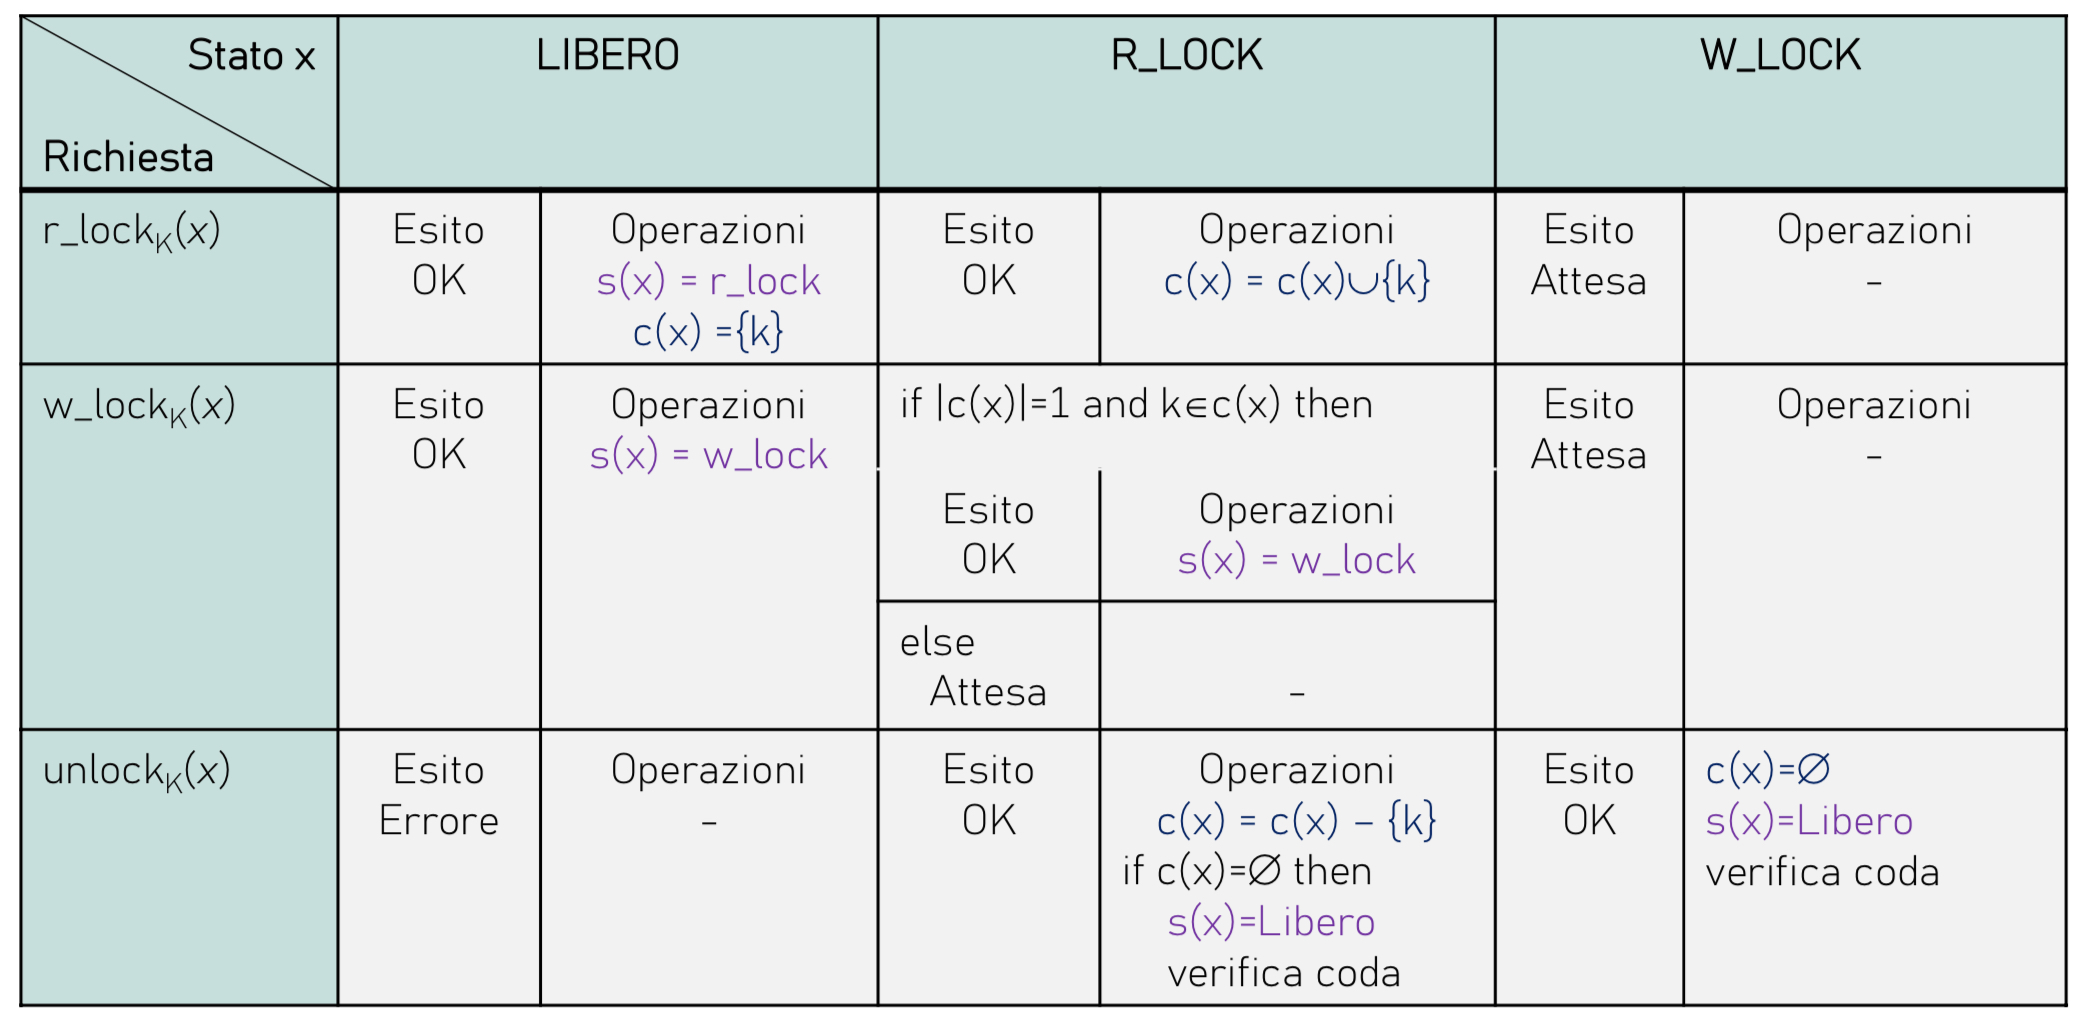
\includegraphics[width=12cm]{img/Tabella_gestione_lock.png}
\end{figure}
\subsection{Serializzabilità}
La regola che garantisce la serializzabilità (\textit{da cui prende il nome il metodo 
2PL}), una transazione dopo aver rilasciato un \verb|LOCK| non può acquisirne altri.
\begin{figure}[H]
  \centering
  \begin{tikzpicture}
    % Disegna gli assi x e y
    \draw[->] (-0.5,0) -- (10,0) node[right] {TEMPO};
    \draw[->] (0,-0.5) -- (0,4) node[above] {LOCK acquisti};
    % Disegno le label delle fasi
    \draw[->] (1.8,2.3) -- (1.8,1.9) node[above, yshift=0.3cm] {I fase: acquisizione};
    \draw[->] (6.2,2.3) -- (6.2,1.9) node[above, yshift=0.3cm] {II fase: rilascio};
    % Disegna il parallelogramma nell'origine
    \draw[red] (0,0) -- (2,2) -- (6,2) -- (8,0);
  \end{tikzpicture}
\end{figure}
\subsection{2PL stretto}
Per rimuovere completamente l'ipotesi di commit-proiezione, una transazione può rilasciare i \verb|LOCK| 
solo quando ha eseguito correttamente un \verb|COMMIT| o 
un \verb|ROLLBACK|.
\begin{figure}[H]
  \centering
  \begin{tikzpicture}
    % Disegna gli assi x e y
    \draw[->] (-0.5,0) -- (10,0) node[right] {TEMPO};
    \draw[->] (0,-0.5) -- (0,4) node[above] {LOCK acquisti};
    % Disegno le label delle fasi
    \draw[->] (1.8,2.3) -- (1.8,1.9) node[above, yshift=0.3cm] {I fase: acquisizione};
    \draw[->] (6.5,3.0) -- (6.5,1.9) node[above, yshift=1.3cm, xshift=0.5cm] {II fase: rilascio};
    % Disegna il parallelogramma nell'origine
    \draw[red] (0,0) -- (2,2) -- (6,2) -- (8,0);
    % cerchio di commit o rollback
    \filldraw[color=red, fill=yellow] (6,2) circle [radius=0.1cm];
    \draw[->] (6,2.8) -- (6,2.3) node[above, yshift=0.4cm,xshift=-1.2cm] {Commit/rollback};
  \end{tikzpicture}
\end{figure}
\subsubsection{Relazione tra 2PL e CSR}
\begin{figure}[H]
  \centering
  \begin{tikzpicture}[scale=1.5]
    % Disegna l'insieme CSR
    \draw[thick, fill=blue!20] (0,0) ellipse (2cm and 1cm) node[xshift=1.5cm] {$CSR$};
    % Disegna il sottoinsieme 2PL in CSR
    \draw[thick, fill=red!20] (-1,0) ellipse (0.9cm and 0.5cm) node {$2PL$};
  \end{tikzpicture}
\end{figure}
\subsection{Blocco critico}
Il blocco critico è una situazione di blocco che si verifica nell'esecuzione di 
transazioni concorrenti quando:
\begin{itemize}
  \item Due transazioni hanno bloccato delle risorse: $t_1$ ha bloccato $r_1$ 
  r $t_2$ ha bloccato $r_2$.
  \item Inoltre $t_1$ è in attesa sulla risorsa $r_2$ e $t_2$ è in attesa sulla risorsa $r_1$.
\end{itemize}
Se il numero medio di tuple per tabella è $n$ e la granularità dei lock è la tupla,
la probabilità che si verifichi un lock tra due transazioni è pari a $\frac{1}{n^2}$.
\subsubsection{Tecniche di risoluzione}
\begin{itemize}
  \item \textbf{Timeout}: una transazione in attesa su una risorsa trascorso il timeout viene abortita.
  \item \textbf{Prevenzione}: 
  \item \begin{itemize}
    \item Una transazione blocca tutte le risorse a cui deve accedere in lettura 
    o scrittura in una sola volta (\textit{o blocca tutto o non blocca nulla}).
    \item Ogni transazione $t_i$ acquisisce un timestamp $\texttt{TS}_i$ all'inizio della sua esecuzione.
    La transazione $t_i$ può attendere una risorsa bloccata da $t_j$ solo se vale una certa 
    condizione sui $\texttt{TS}$ ($\texttt{TS}_i < \texttt{TS}_j$) altrimenti viene abortita e fatta ripartire con lo stesso $TS$.
  \end{itemize}
  \item \textbf{Rilevamento}: si esegue un'analisi periodica della tabella di \verb|LOCK| per rilevare la 
  presenza di un blocco critico (\textit{corrisponde ad un ciclo nel grafo 
  delle relazioni di attesa}). Questa tecnica è quella più frequentemente adottata dai sistemi 
  reali.
\end{itemize}
La scelta di gestire i lock in lettura come lock condivisi produce un ulteriore problema chiamato starvation 
che tuttavia nel contesto delle DBMS risulta poco probabile.

Se una risorsa $x$ viene costantemente bloccata da una sequenza di transazioni che acquisiscono 
\verb|r_lock| su $x$, un'eventuale transazione in attesa di scrivere su $x$ viene 
bloccata per un lungo periodo fino alla fine della sequenza di letture.

Anche se poco probabile tale evenienza può essere scongiurata con tecniche 
simili a quanto visto per il blocco critico. In particolare è possibile 
analizzare la tabella delle relazioni di attesa e verificare da quanto tempo 
le transazioni stanno attendendo la risorsa e di conseguenza sospendere 
temporaneamente la concessione di lock in lettura condivisi per consentire la scrittura da parte 
della transazione in attesa.

Poiché risulta molto oneroso per il sistema gestire l'esecuzione concorrente di 
transazioni con conseguente diminuzione delle prestazioni del sistema, SQL 
prevede la possibilità di rinunciare in tutto o in parte al controllo di concorrenza per aumentare le prestazioni 
del sistema.

Ciò significa che è possibile a livello di singola transazione decidere di tollerare alcune 
anomalie di esecuzione concorrente.
\subsection{Gestione della concorrenza in SQL}
Tutti i livelli richiedono 2PL stretto per le scritture.
\begin{itemize}
  \item \verb|serializable|: lo richiede anche per le letture e applica 
  il lock di predicato per evitare l'inserimento fantasma.
  \item \verb|repeatable read|: applica 2PL stretto per tutti i lock in 
  lettura applicati a livello di tupla e non di tabella. Consente inserimenti 
  e quindi non evita l'anomalia di inserimento fantasma.
  \item \verb|read committed|: richiede lock condivisi per le letture ma non il
  2PL stretto.
  \item \verb|read uncommitted|: non applica lock in lettura.
\end{itemize}
\chapter{Ottimizzazione di interrogazioni}
Ogni interrogazione sottomessa al DBMS viene espressa in un linguaggio dichiarativo,
è quindi necessario trovare un equivalente espressione in linguaggio procedurale 
(\textit{ad esempio in algebra relazionale}) per generare un piano di esecuzione.

L'espressione algebrica va ottimizzata rispetto alle caratteristiche del DBMS a livello 
fisico e della base di dati corrente.
\section{Ottimizzazione}
L'ottimizzazione avviene secondo i seguenti passi:
\begin{figure}[H]
  \centering
  \begin{tikzpicture}[node distance=1.5cm, auto]
    % definisci i nodi
    \node (rect1) [ellipse, draw, fill=blue!30, minimum height=1cm, minimum width=3cm] {Query};
    \node (rect2) [rectangle, draw, fill=red!30, below of=rect1, minimum height=1cm, minimum width=3cm]  {Analisi lessicale e sintattica};
    \node (rect3) [rectangle, draw, fill=green!30, below of=rect2, minimum height=1cm, minimum width=3cm]  {Ottimizzazione algebrica};
    \node (rect4) [rectangle, draw, fill=orange!30, below of=rect3, minimum height=1cm, minimum width=3cm]  {Ottimizzazione dipendenza e metodi d'accesso};
    \node (rect5) [rectangle, draw, fill=yellow!30, below of=rect4, minimum height=1cm, minimum width=3cm]  {Generazione del codice};
    \node (rect6) [rectangle, draw, fill=purple!30, below of=rect5, minimum height=1cm, minimum width=3cm]  {Codice eseguibile};
    \node (cyl) [cylinder, below right of=rect4, xshift=5cm, shape border rotate=90, draw, fill=gray!30, minimum height=4cm, minimum width=2cm, aspect=0.3] {\begin{tabular}{c} Profili \\ delle \\ tabelle \end{tabular}};
  
    % definisci i collegamenti
    \draw [->] (rect1) -- (rect2);
    \draw [->] (rect2) -- (rect3);
    \draw [->] (rect3) -- (rect4);
    \draw [->] (rect4) -- (rect5);
    \draw [->] (rect5) -- (rect6);
    \draw [<->] (rect4.east) -- (cyl.west);
  \end{tikzpicture}
\end{figure}
L'ottimizzazione algebrica di basa fondamentalmente sulle regole di ottimizzazione 
già note dell'algebra relazionale:
\begin{itemize}
  \item Anticipo delle selezioni;
  \item Anticipo delle proiezioni.
\end{itemize}
\section{Ottimizzazione dipendente dai metodi di accesso}
Le operazioni tipiche di accesso supportate dai DBMS sono:
\begin{itemize}
  \item Scansione (\textit{scan}) delle tuple di una relazione.
  \item Ordinamento di un insieme di tuple.
  \item Accesso diretto alle tuple attraverso indice.
  \item Diverse implementazioni del join.
\end{itemize}
\subsection{Scansione}
Una operazione di \verb|scan| opera contestualmente altre operazioni, tra cui:
\begin{itemize}
  \item \verb|scan| e \verb|proiezione| senza eliminazione di duplicati.
  \item \verb|scan| e \verb|selezione| in base ad un predicato semplice.
  \item \verb|scan| e inserimento, cancellazione o modifica.
\end{itemize}
Il costo di una scansione sulla relazione $\verb|R|$ è $\verb|NP(R)|$, dove $\verb|NP(R)|$
è il numero di pagine date dalla relazione \verb|R|.
\subsection{Ordinamento}
L'ordinamento viene utilizzato per ordinare il risultato di un'interrogazione (\textit{con la clausola} \verb|order by|),
eliminare duplicati (\verb|select distinct|) e raggruppare tuple (\verb|group by|).

L'ordinamento su memoria secondaria viene eseguito tramite l'algoritmo \textbf{Z-way Merge Sort} che si suddivide 
in due fasi:
\begin{itemize}
  \item Sort interno: si leggono una alla volta le pagine della tabella; le tuple 
  di ogni pagina vengono ordinate facendo uso di un algoritmo di sort interno. 
  Ogni pagina così ordinata, viene detta anche  ``run'', viene scritta su memoria secondaria in un file temporaneo.
  \item Merge: applicando uno o più passi di fusione, le run vengono unite a produrre un'unica run.
\end{itemize}
\subsubsection{Z-way Sort-Merge}
\begin{figure}[H]
  \centering
  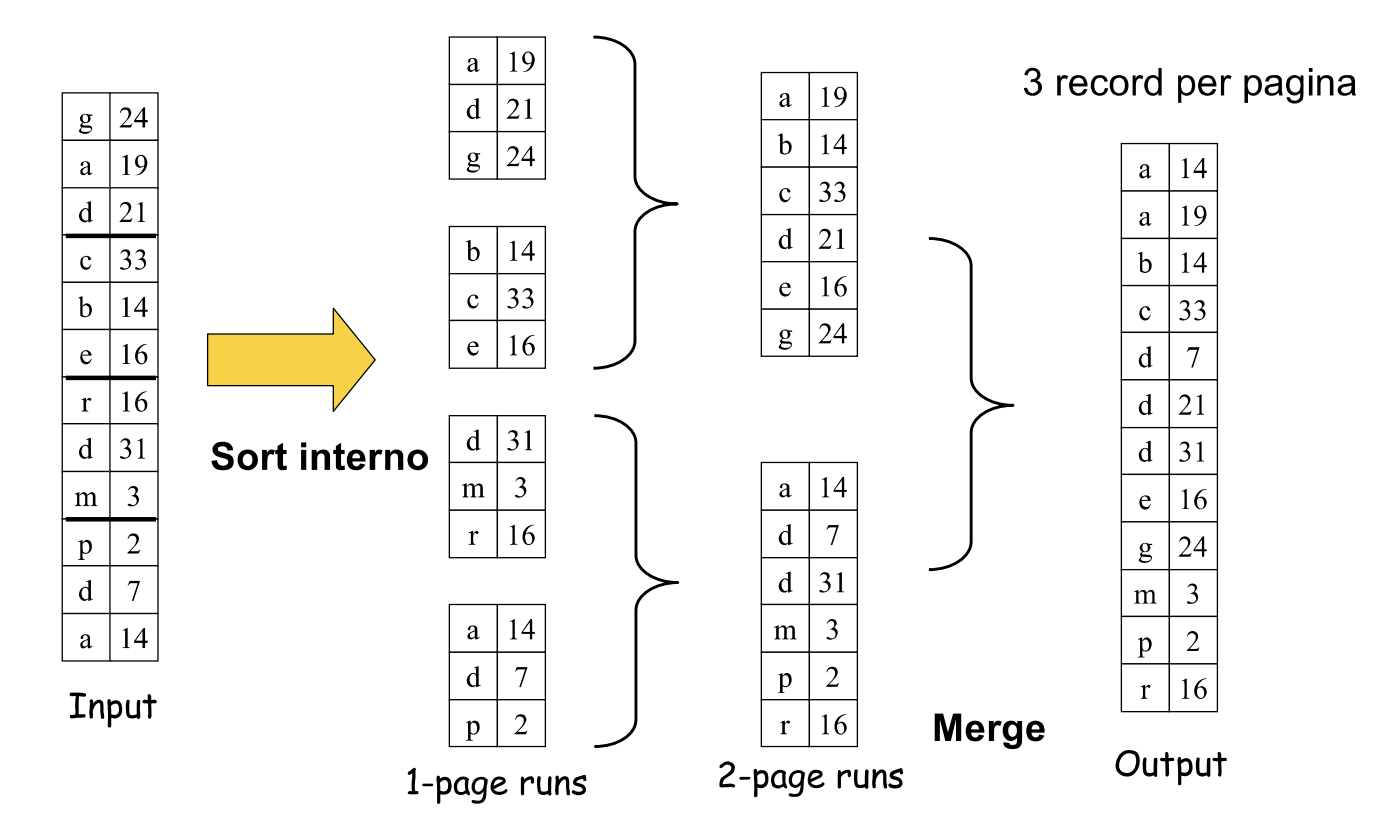
\includegraphics[width=10cm]{img/z-way-merge-sort.png}
\end{figure}
Il costo, considerando solo il numero di accessi a memoria secondaria è 
\[
  2 \cdot \texttt{NP} \cdot \left( \lceil \log_2 \texttt{NP}\rceil + 1\right)
\]
Dove la moltiplicazione per due considera lettura e scrittura.
\subsection{Accesso diretto via indice}
Le interrogazioni che fanno uso dell'indice:
\begin{itemize}
  \item Selezioni con condizione atomica di uguaglianza $(A = v)$ richiedono indice hash o
  B+-Tree.
  \item Selezioni con condizioni di range $(A >=v_1\, \texttt{AND} \, A <=v_2)$ richiedono indice B+-Tree.
  \item Le selezioni con condizione costruita da una congiunzione di condizioni di uguaglianza $(A >=v_1\, \texttt{AND} \, B <=v_2)$:
  in questo caso si sceglie per quale delle condizioni di uguaglianza utilizzare l'indice; la 
  scelta ricade sulla condizione più selettiva. L'altra si verifica direttamente sulle pagine dati.
  \item Le selezioni con condizione da disgiunzione di condizioni di uguaglianza, così composte $(A >=v_1\, \texttt{ } \, B <=v_2)$:
  in questo caso è possibile utilizzare più indici in parallelo, facendo un merge dei risultati eliminando i duplicati oppure,
  se manca anche solo uno degli indici, è necessario eseguire una scansione sequenziale.
\end{itemize}
\section{Algoritmi per il join}
Il join è l'operazione più gravoso per un DBMS, le implementazioni più diffuse 
si riconducono ai seguenti operatori fisici:
\begin{itemize}
  \item Nested Loop Join.
  \item Merge Scan Join.
  \item Hash-based Join.
\end{itemize}
Si noti, benché logicamente il join sia commutativo, dal punto di vista fisico 
vi sia una chiara distinzione, che influenza anche le prestazioni, tra operando sinistro e operando 
destro. Per semplicità nel seguito parliamo di relazione esterna e relazione 
interna per riferirci agli input del join, ma va ricordato che in generale l'input 
può derivare all'applicazione di altri operatori.
\subsection{Nested-Loop Join}
Date due relazioni in input $\mathcal{R}$ e $\mathcal{S}$ tra cui sono definiti i predicati di join 
$PJ$, e supponendo che $\mathcal{R}$ sia la relazione esterna, l'algoritmo opera come segue.
\begin{lstlisting}[mathescape]
  per ogni tupla $t_\mathcal{R} \in \mathcal{R}${
    per ogni tupla $t_\mathcal{S} \in \mathcal{R}${
      if (($t_\mathcal{R},T_\mathcal{S}$) soddisfa PJ)
        then aggiungi ($t_\mathcal{R},T_\mathcal{S}$) al risultato
    }
  }
\end{lstlisting}
Il costo di esecuzione dipende dallo spazio a disposizione nei buffer.
Nel caso base in cui vi sia un buffer per $\mathcal{R}$ e un buffer per $\mathcal{S}$
allora bisogna leggere una volta $\mathcal{R}$ e $\texttt{NR}(\mathcal{R})$ volte $\mathcal{S}$,
ovvero tante vole quante sono le tuple della relazione esterna.
Per un totale di 
\[
  \texttt{NP}(\mathcal{R}) + \texttt{NR}(\mathcal{R}) \cdot \texttt{NP}(\mathcal{S})
\]
Se è possibile allocare $\texttt{NP}(\mathcal{S})$ buffer per la relazione interna il costo si riduce a 
$\texttt{NP}(\mathcal{R}) + \texttt{NP}(\mathcal{S})$.
\subsubsection{Nested-Loop Join con indice B+-Tree}
Data una tupla della relazione esterna $\mathcal{R}$, la scansione completa della relazione interna 
$\mathcal{S}$ può essere sostituita da una scansione basata su un indice costruito sugli attributi 
di join di $\mathcal{S}$.

Nel caso in cui vi sia un buffer per $\mathcal{R}$ e un buffer per $\mathcal{S}$, bisogna 
leggere una volta $\mathcal{R}$ e accedere $\texttt{NR}(\mathcal{R})$ volte a $\mathcal{S}$, 
ovvero tante volte quante sono le tuple della relazione esterna, per un totale di 
\[
  \texttt{NP}(\mathcal{R}) + \texttt{NR}(\mathcal{R}) \cdot \left((\texttt{Prof indice} + \frac{\texttt{NR}(\mathcal{S})}{\text{VAL}(\mathcal{A}, \mathcal{S})}\right)
\]
dove: \verb|VAL|$(\mathcal{A}, \mathcal{S})$ rappresenta il numero di valori distinti dall'attributo di $\mathcal{A}$
che compaiono nella relazione $\mathcal{S}$.
\subsubsection{Block Nested-Loop Join}
Si tratta di una variante che bufferizza le righe lette della tabella esterna per ridurre il numero 
di volte che deve essere letta nel ciclo interno.

Il costo di esecuzione dipende dallo spazio a disposizione nei buffer. Nel caso 
base vi sia un buffer per $\mathcal{R}$ e un buffer per $\mathcal{S}$ allora bisogna 
leggere una volta $\mathcal{R}$ e $\texttt{NP}(\mathcal{R})$ volte $\mathcal{S}$, ovvero 
tante volte quanti sono i blocchi della relazione esterna, per un totale di 
$\texttt{NP}(\mathcal{R}) + \texttt{NP}(\mathcal{R}) \cdot \texttt{NP}(\mathcal{S})$ accessi a memoria secondaria.

Se è possibile allocare $\texttt{NP}(\mathcal{S})$ buffer per la relazione interna il costo si riduce a 
$\texttt{NP}(\mathcal{R}) + \texttt{NP}(\mathcal{S})$.
\subsection{Merge-Scan Join}
Il Merge-Scan Join è applicabile quando entrambi gli insiemi di tuple in input sono ordinati 
sugli attributi di join e il join e un equi-join.

Ciò accade se per entrambe le relazioni di input $\mathcal{R}$ e $\mathcal{S}$ 
vale almeno una delle seguenti condizioni:
\begin{itemize}
  \item La relazione è fisicamente ordinata sugli attributi di join (\textit{file 
  sequenziale ordinato come struttura fisica}).
  \item Esiste un indice sugli attributi di join della tabella che consente una scansione ordinata 
  delle tuple.
\end{itemize}
La logica dell'algoritmo sfrutta il fatto che entrambi gli input siano ordinati 
per evitare di fare inutili confronti, il che fa sì che il numero di letture totali 
sia dell'ordine di $\texttt{NP}(\mathcal{R}) + \texttt{NP}(\mathcal{S})$ se si accede sequenzialmente alle 
due relazioni ordinate fisicamente.

Con indici B+-Tree su entrambe le relazioni il costo può arrivare al massimo a 
$\texttt{NR}(\mathcal{R}) + \texttt{NR}(\mathcal{S})$.
Con una relazione ordinata e un solo indice al massimo a $\texttt{NP}(\mathcal{R}) + \texttt{NR}(\mathcal{S})$ o viceversa.
\subsection{Hash-based Join}
L'algoritmo di Hash Join, applicabile solo in caso di equi-join, non richiede nè la presenza di 
indici nè input ordinati, e risulta particolarmente vantaggioso in caso di relazioni molto grandi.
L'idea su cui si basa l'Hash Join è semplice:
si suppone di avere a disposizione una funzione hash $h$, che viene applicata agli attributi di join 
delle due relazioni
\begin{itemize}
  \item se $t_\mathcal{R}$ e $t_\mathcal{S}$ sono due tuple di $\mathcal{R}$ e 
  $\mathcal{S}$, allora è possibile che sia $t_\mathcal{R}.J = t_\mathcal{S}.J$
  solo se $h(t_\mathcal{R}.J) = h(t_\mathcal{S}.J)$.
  \item Se, viceversa, $t_\mathcal{R}.J \not= t_\mathcal{S}.J$
  allora $h(t_\mathcal{R}.J) \not= h(t_\mathcal{S}.J)$.
\end{itemize}
A partire da questa idea si hanno diverse implementazioni. che hanno in comune il fatto che $\mathcal{R}$ e 
$\mathcal{S}$ vengono partizionate sulla base dei valori della funzione di hash $h$, e che 
la ricerca di matching tuples avviene solo tra partizioni relative allo stesso valore di $h$.

Il costo può essere così valutato:
\begin{itemize}
  \item costruzione hash-map: $\texttt{NP}(\mathcal{R}) + \texttt{NP}(\mathcal{S})$.
  \item Accesso alle matching tuples che nel  caso pessimo può costare: $\texttt{NP}(\mathcal{R}) \cdot \texttt{NP}(\mathcal{S})$.
\end{itemize}
Dipende però fortemente dal numero di buffer a disposizione e dalla distribuzione dei valori degli attributi di join.
\subsection{Scelta finale del piano di esecuzione}
Data una espressione ottimizzata in algebra, si generano tutti i possibili piani di esecuzione (\textit{alberi}) 
alternativi (\textit{o sottoinsieme di questi}) ottenuti considerando le seguenti dimensioni:
\begin{itemize}
  \item Operatori alternativi applicabili per l'accesso ai dati: ad esempio, \verb|scan| sequenziale o via indice.
  \item Operatori alternativi applicabili nei nodi: ad esempio, \verb|nested-loop join| o \verb|hash-based| \verb|join|.
  \item L'ordine delle operazioni da compiere (\textit{associatività}.)
\end{itemize}
Si valuta con formule approssimate il costo di ogni alternativa in termini di accessi a 
memoria secondaria richiesti (\textit{stima}) e si sceglia l'albero con costo approssimato minimo.

Nella valutazione delle stime di costo si tiene conto del profilo delle relazioni, solitamente 
memorizzato nella Data Directory e contenente per ogni relazione $\mathcal{T}$:
\begin{itemize}
  \item Stima della cardinalità: \verb|CARD|$(\mathcal{T})$;
  \item Stima della dimensione di una tupla: \verb|SIZE|$(\mathcal{T})$;
  \item Stima della dimensione di ciascun attributo $(\mathcal{A})$: \verb|SIZE|$(\mathcal{A},\mathcal{T})$;
  \item Stima del numero di valori distinti per ogni attributo $(\mathcal{A})$: \verb|VAL|$(\mathcal{A},\mathcal{T})$;
  \item Stima del valore massimo e minimo per ogni attributo $\mathcal{A}$:
  \verb|MAX|$(\mathcal{A},\mathcal{T})$ e \verb|MIN|$(\mathcal{A},\mathcal{T})$;
\end{itemize}
\end{document}